% Options for packages loaded elsewhere
\PassOptionsToPackage{unicode}{hyperref}
\PassOptionsToPackage{hyphens}{url}
%
\documentclass[
]{article}
\usepackage{amsmath,amssymb}
\usepackage{lmodern}
\usepackage{ifxetex,ifluatex}
\ifnum 0\ifxetex 1\fi\ifluatex 1\fi=0 % if pdftex
  \usepackage[T1]{fontenc}
  \usepackage[utf8]{inputenc}
  \usepackage{textcomp} % provide euro and other symbols
\else % if luatex or xetex
  \usepackage{unicode-math}
  \defaultfontfeatures{Scale=MatchLowercase}
  \defaultfontfeatures[\rmfamily]{Ligatures=TeX,Scale=1}
\fi
% Use upquote if available, for straight quotes in verbatim environments
\IfFileExists{upquote.sty}{\usepackage{upquote}}{}
\IfFileExists{microtype.sty}{% use microtype if available
  \usepackage[]{microtype}
  \UseMicrotypeSet[protrusion]{basicmath} % disable protrusion for tt fonts
}{}
\makeatletter
\@ifundefined{KOMAClassName}{% if non-KOMA class
  \IfFileExists{parskip.sty}{%
    \usepackage{parskip}
  }{% else
    \setlength{\parindent}{0pt}
    \setlength{\parskip}{6pt plus 2pt minus 1pt}}
}{% if KOMA class
  \KOMAoptions{parskip=half}}
\makeatother
\usepackage{xcolor}
\IfFileExists{xurl.sty}{\usepackage{xurl}}{} % add URL line breaks if available
\IfFileExists{bookmark.sty}{\usepackage{bookmark}}{\usepackage{hyperref}}
\hypersetup{
  pdftitle={100-day mission: Model description},
  hidelinks,
  pdfcreator={LaTeX via pandoc}}
\urlstyle{same} % disable monospaced font for URLs
\usepackage[margin=1in]{geometry}
\usepackage{longtable,booktabs,array}
\usepackage{calc} % for calculating minipage widths
% Correct order of tables after \paragraph or \subparagraph
\usepackage{etoolbox}
\makeatletter
\patchcmd\longtable{\par}{\if@noskipsec\mbox{}\fi\par}{}{}
\makeatother
% Allow footnotes in longtable head/foot
\IfFileExists{footnotehyper.sty}{\usepackage{footnotehyper}}{\usepackage{footnote}}
\makesavenoteenv{longtable}
\usepackage{graphicx}
\makeatletter
\def\maxwidth{\ifdim\Gin@nat@width>\linewidth\linewidth\else\Gin@nat@width\fi}
\def\maxheight{\ifdim\Gin@nat@height>\textheight\textheight\else\Gin@nat@height\fi}
\makeatother
% Scale images if necessary, so that they will not overflow the page
% margins by default, and it is still possible to overwrite the defaults
% using explicit options in \includegraphics[width, height, ...]{}
\setkeys{Gin}{width=\maxwidth,height=\maxheight,keepaspectratio}
% Set default figure placement to htbp
\makeatletter
\def\fps@figure{htbp}
\makeatother
\setlength{\emergencystretch}{3em} % prevent overfull lines
\providecommand{\tightlist}{%
  \setlength{\itemsep}{0pt}\setlength{\parskip}{0pt}}
\setcounter{secnumdepth}{5}
%%%% pandoc-fignos: required package
\usepackage{caption}
\usepackage{xcolor}
\usepackage[round]{natbib}

%% pandoc-fignos: environment to disable figure caption prefixes
\makeatletter
\newcounter{figno}
\newenvironment{fignos:no-prefix-figure-caption}{
  \caption@ifcompatibility{}{
    \let\oldthefigure\thefigure
    \let\oldtheHfigure\theHfigure
    \renewcommand{\thefigure}{figno:\thefigno}
    \renewcommand{\theHfigure}{figno:\thefigno}
    \stepcounter{figno}
    \captionsetup{labelformat=empty}
  }
}{
  \caption@ifcompatibility{}{
    \captionsetup{labelformat=default}
    \let\thefigure\oldthefigure
    \let\theHfigure\oldtheHfigure
    \addtocounter{figure}{-1}
  }
}
\makeatother
\usepackage{float}
\usepackage{booktabs}
\usepackage{longtable}
\usepackage{array}
\usepackage{multirow}
\usepackage{wrapfig}
\usepackage{colortbl}
\usepackage{pdflscape}
\usepackage{tabu}
\usepackage{threeparttable}
\usepackage{threeparttablex}
\usepackage[normalem]{ulem}
\usepackage{makecell}
\usepackage{xcolor}
\ifluatex
  \usepackage{selnolig}  % disable illegal ligatures
\fi
\newlength{\cslhangindent}
\setlength{\cslhangindent}{1.5em}
\newlength{\csllabelwidth}
\setlength{\csllabelwidth}{3em}
\newenvironment{CSLReferences}[2] % #1 hanging-ident, #2 entry spacing
 {% don't indent paragraphs
  \setlength{\parindent}{0pt}
  % turn on hanging indent if param 1 is 1
  \ifodd #1 \everypar{\setlength{\hangindent}{\cslhangindent}}\ignorespaces\fi
  % set entry spacing
  \ifnum #2 > 0
  \setlength{\parskip}{#2\baselineskip}
  \fi
 }%
 {}
\usepackage{calc}
\newcommand{\CSLBlock}[1]{#1\hfill\break}
\newcommand{\CSLLeftMargin}[1]{\parbox[t]{\csllabelwidth}{#1}}
\newcommand{\CSLRightInline}[1]{\parbox[t]{\linewidth - \csllabelwidth}{#1}\break}
\newcommand{\CSLIndent}[1]{\hspace{\cslhangindent}#1}

\title{100-day mission: Model description}
\author{}
\date{\vspace{-2.5em}}

\begin{document}
\maketitle

\hypertarget{simulation-rules}{%
\section{Simulation rules}\label{simulation-rules}}

\begin{itemize}
\tightlist
\item
  Countries are instantiated with two random variables: the response time, and their importation time
\item
  The response time is the time at which the reporting country reports having seen X hospital cases, where X is a random number between 1 and 20
\item
  The importation time is a random number between 0 and 20 days, where 0 days would be equivalent to the spillover, or origin, country
\item
  The simulation starts at the minimum between the response time and the importation time
\item
  At the response time, the BPSV, if present, is given to people aged 65 and older; testing begins; social distancing begins; economic closures, if in use, are implemented
\item
  At the importation time, five people are moved from compartment S to compartment E
\item
  If closures are being implemented, the rules in Tables \ref{tab:rulesreactive} and \ref{tab:ruleselimination} are followed
\item
  The SARS-X--specific vaccine is rolled out starting on day 107 or 372 after the response time, depending on the investment assumption
\item
  All people aged 15 and over are eligible for vaccination, and we assume 80\% take it up
\item
  Distribution rate increases linearly to a maximum of 1\% of the population per day, at which is stays until 80\% coverage is reached
\item
  When vaccine rollout is complete, closures, testing and social distancing end
\item
  When the doubling time is more than 30 days and there are fewer than 1,000 people in hospital, the simulation ends.
\end{itemize}

\begin{longtable}[]{@{}
  >{\raggedright\arraybackslash}p{(\columnwidth - 6\tabcolsep) * \real{0.25}}
  >{\raggedright\arraybackslash}p{(\columnwidth - 6\tabcolsep) * \real{0.25}}
  >{\raggedright\arraybackslash}p{(\columnwidth - 6\tabcolsep) * \real{0.25}}
  >{\raggedright\arraybackslash}p{(\columnwidth - 6\tabcolsep) * \real{0.25}}@{}}
\caption{\label{tab:rulesreactive} State transition rules for reactive closure strategies}\tabularnewline
\toprule
From/to & No closures & Light closures & Heavy closures \\
\midrule
\endfirsthead
\toprule
From/to & No closures & Light closures & Heavy closures \\
\midrule
\endhead
\textbf{No closures} & & & t = response time OR Hospital occupancy \textgreater{} 95\% capacity \\
\textbf{Light closures} & (Growth rate \textless{} 0.025 OR Hospital occupancy \textless{} 25\% capacity) AND vaccine rollout complete OR \(R_t(M(\textbf{1})) < 1\) & & Hospital occupancy \textgreater{} 95\% capacity \\
\textbf{Heavy closures} & & Hospital occupancy \textless{} 25\% capacity AND t \textgreater{} 7 + last change time & \\
\bottomrule
\end{longtable}

\begin{longtable}[]{@{}
  >{\raggedright\arraybackslash}p{(\columnwidth - 6\tabcolsep) * \real{0.25}}
  >{\raggedright\arraybackslash}p{(\columnwidth - 6\tabcolsep) * \real{0.25}}
  >{\raggedright\arraybackslash}p{(\columnwidth - 6\tabcolsep) * \real{0.25}}
  >{\raggedright\arraybackslash}p{(\columnwidth - 6\tabcolsep) * \real{0.25}}@{}}
\caption{\label{tab:ruleselimination} State transition rules for the elimination strategy}\tabularnewline
\toprule
From/to & No closures & Light closures & Heavy closures \\
\midrule
\endfirsthead
\toprule
From/to & No closures & Light closures & Heavy closures \\
\midrule
\endhead
\textbf{No closures} & & & t = response time OR Hospital occupancy \textgreater{} 95\% capacity \\
\textbf{Light closures} & Vaccine rollout complete OR \(R_t(M(\textbf{1})) < 1\) & & \(R_t > 1.2\) \\
\textbf{Heavy closures} & Vaccine rollout complete OR \(R_t(M(\textbf{1})) < 1\) & \(R_t(M_{\text{light closure}}) < 0.95\) AND t \textgreater{} 7 + last change time & \\
\bottomrule
\end{longtable}

\hypertarget{socio-economic-costs}{%
\section{Socio-economic costs}\label{socio-economic-costs}}

We assign monetary values to YLLs and to years of education in order to add health and education costs of mitigation strategies to the costs of economic closures. We define the total socio-economic costs TSC of an epidemic as the sum of the individual costs:

\begin{equation}
\text{TSC} = K_1\text{VLY} + K_2 + K_3\text{VSY},
\label{eq:swf}
\end{equation}

where \(K_1\) is the number of discounted life years lost and VLY the value of a discounted life year; \(K_2\) is the lost GDP over the period due to reduced economic activity; and \(K_3\) is the number of school years lost and VSY the value of one school year.

\hypertarget{lost-lives}{%
\subsection{Lost lives}\label{lost-lives}}

To value lives lost, we make use of the expected remaining life years per age group (Global Burden of Disease Collaborative Network 2021). These are used to estimate the expected number of years of life lost per death, and to estimate the value of a life year. We map the remaining life expectancy \(\tilde{l}_a\) for the GBD age groups \(a\) to \(l_g\) for the model age groups \(g\) as a population-weighted average, taking into account the size of each age group, \(`\tilde{N}_a`\). For the expected number of life years lost per death, we take into account also the probability to die given infection, \(P(D|I,a)\):

\begin{verbatim}
l_g^{\text{(death)}} = \frac{\sum_{a\in g}N_a\tilde{l}_aP(D|I,a)}{\sum_{a\in g}N_aP(D|I,a)}; 
\end{verbatim}

\begin{verbatim}
l_g^{\text{(life)}} = \frac{\sum_{a\in g}N_a\tilde{l}_a}{\sum_{a\in g}\tilde{N}_a}; 
\end{verbatim}

Expected life years remaining with discounting taken into account can be written

\begin{verbatim}
\hat{l}_g=\sum_{y=1}^{l_g}\frac{1}{(1+r)^{y}}
\end{verbatim}

for discount rate \(r>0\). The discounted number of years lost given \(D_g\) deaths due to COVID-19 for each age group is

\begin{verbatim}
K_1=\sum_gD_g\hat{l}_g^{\text{(death)}}.
\end{verbatim}

The VLY used by policy makers should reflect the value that members of the society place on reductions of their own mortality.
We rely on the intrinsic rather than instrumental interpretation of the valuation of life (Cutler and Summers 2020), and we use existing estimates of the value of a statistical life (VSL) to estimate VLY. We interpret the VSL as a population-weighted average (Ananthapavan et al. 2021; Robinson, Sullivan, and Shogren 2021), where each age group has a VSL defined by the number of expected life years remaining, and where each discounted year has the same value:

\begin{equation}
\text{VSL}=\frac{\sum_gN_g\hat{l}_g^{\text{(life)}}}{\sum_gN_g}\text{VLY}.
\end{equation}

\hypertarget{lost-economic-activity}{%
\subsection{Lost economic activity}\label{lost-economic-activity}}

We measure the cost of economic closures in terms of lost gross value added (GVA): the GDP generated by an economic configuration is the maximum GVA (denoted \(y_j\) for each sector \(j\)) multiplied by the respective sector openings, summed over the period (\(\tau\) days). The maximum possible GDP (which is with no closures) is

\[Y_0=\frac{\tau}{365}\sum_{j=1}^{m_S}y_j\]

for \(m_S\) sectors, and we use pre-pandemic GVA to define the maximum possible values.

All economic sectors contribute GVA according to the level they are open for production, except for the education sector which contributes its maximum possible GVA, \(y_{\text{ed}}\). \(x_{j}(t)\) is the proportion of the workforce contributing to economic production in sector \(j\) out of the total workforce \(N_j\) on day \(t\). The workforce can be additionally depleted due to self isolation, sickness, hospitalisation and death, leaving a smaller fraction (\(`\hat{x}_{j}(t)`\)) to contribute to production.

\begin{verbatim}
\hat{x}_{j}(t)=x_{j}(t) - \left((1-x_{j}(t))p_j^{23}(t)  + (1-x_{j}(t)(1-q_j))p_j^{22}(t)\right)/N_j
\end{verbatim}

where \(q_j\) is the fraction of the sector working from home. \(p_j^{23}(t)\) represents worker sickness and death:

\[p_j^{23}(t)=\sum_{v=0}^{m_V}\left(\left(1-p^H_{j,v}\right)p^1p^{19}I_{j,v}^{s}+p^H_{j,v}p^1I_{j,v}^{s}+H_{j,v}+D_{j,v}\right),\]

with \(m_V=2\) vaccines and \(p_j^{22}(t)\) represents output from asymptomatic self-isolating workers:

\[p_j^{22}(t)=p^2(t)p^{18}I_{j}^{a}.\]

\(p^{18}\) is the number of days spent in self isolation per day of infectiousness (e.g.~suppose the average infectious period is four days and mandatory self-isolation time is ten days, then \(p^{19}=2.5\) and \(p^{18}=p^{19}T^{I^s}/T^{I^a:R}\), where \(T^{I^s}\) and \(T^{I^a:R}\) are expected infectious periods for symptomatic and asymptomatic, respectively). \(p^1\) is compliance with the requirement to self isolate and \(p^2(t)\) is the fraction of cases identified. Other notations are vaccine status \(v\), infectious and asymptomatic \(I_{j,v}^{a}\), infectious and symptomatic \(I_{j,v}^{s}\), hospitalised \(H\), deceased \(D\), and probability to be hospitalised \(p^H\).

Then the total GDP is

\begin{verbatim}
Y =  \frac{1 }{365} \sum_{j\neq\text{ed}}^{m_S}y_j\int_{t=0}^{\tau}\hat{x}_{j}(t)dt + \frac{\tau }{365}{y_\text{ed}},
\end{verbatim}

and the GDP loss compared to the maximum is

\[K_2=Y_0-Y.\]

\hypertarget{lost-education}{%
\subsection{Lost education}\label{lost-education}}

The loss due to school closure is

\[K_3 =  \frac{1 }{365} \int_{t=0}^{\tau}\left(p^{14}(t)N_{j_{\text{school}}} + (1-p^{14}(t))p^{25}(t)  +(1-2p^{14}(t))p^{24}(t)\right)dt,\]

where \(p^{14}(t)\) is the effective amount of education lost per student at time \(t\) due to school closure:
\[p^{14}(t) = (1-p^{16})(1-x_{\text{ed}}(t)),\]
\(N_{j_{\text{school}}}\) is the total number of students, \(p^{16}\) is relative effectiveness of remote education and \(x_{\text{ed}}(t)\) is the openness of schools, \(p^{25}(t)\) represents education lost due to student sickness with COVID-19:

\[p^{25}(t)=\sum_{v=0}^{m_V}\left((1-p^H_{j_{\text{school}},v})p^1p^{19}I_{j_{\text{school}},v}^{s}+p^H_{j_{\text{school}},v}p^1I_{j_{\text{school}},v}^{s}+H_{j_{\text{school}},v}\right),\]

\(p^{18}\) is the number of days spent in self isolation per day of infectiousness (e.g.~suppose the average infectious period is four days and mandatory self-isolation time is ten days, then \(p^{19}=2.5\) and \(p^{18}=p^{19}T^{I^s}/T^{I^a:R}\), where \(T^{I^s}\) and \(T^{I^a:R}\) are expected infectious periods for symptomatic and asymptomatic, respectively), and \(p^{24}(t)\) represents education lost due to asymptomatic self isolation (which comes at a cost only when schools are open):

\[p^{24}(t)=p^2(t)p^{18}I_{j_{\text{school}}}^{a}.\]

For the value of a year of education, we use the method of (Psacharopoulos, Collis, and Patrinos 2021).

\[\text{VSY} =  p^{12}\cdot p^{13}\cdot p^{15}.\]

\(p^{12}\) is the present value of lost earnings:

\[p^{12} = \frac{1}{N_{j_{\text{school}}}}\sum_{a\in j_{\text{school}}}\tilde{N}_a\left( \frac{1-(1+r)^{-(m_Y+20-a)}}{r} -  \frac{1-(1+r)^{-(20-a)}}{r}\right)\]

for discount rate \(r=0.03\), number \(\tilde{N}_a\) students currently age \(a\), and expected number of years of work \(m_Y=45\). \(p^{13}\) is mean annual earnings, \(p^{15}=0.08\) is the rate of return for one year.

The value \(p^{16}\) represents the effectiveness of remote teaching, which we sample as a standard uniform random variable. We note that no strong predictors of effectiveness of remote teaching have been identified (Patrinos 2023). We assume that losses are linear in duration of school closure, although there is not consensus even on this (Betthäuser, Bach-Mortensen, and Engzell 2023). Important factors to include in future work might be those relating to parental circumstances including education level, engagement and socio-economic status (Moscoviz and Evans 2022). However, these factors might be more pertinent to intra- rather than international modelling.

\hypertarget{epi-model}{%
\section{Epi model}\label{epi-model}}

\hypertarget{ordinary-differential-equations}{%
\subsection{Ordinary differential equations}\label{ordinary-differential-equations}}

\begin{align}
\frac{dS_{j,v}}{dt} & = \sum_{u=0}^{v-1}k^9S_{j,u}^{c_v} - \left( k_{j,v}^{1}(t) + \sum_{u=v+1}^{{m_V}}k_{j,v}^{10,c_u}(t) \right)S_{j,v} \\
\frac{dS_{j,u}^{c_v}}{dt} & = k_{j,u}^{10,c_v}(t)S_{j,u} -\left( k_{j,u}^{1}(t) + k^9 \right)S_{j,u}^{c_v}  \\
\frac{dE_{j,v}}{dt} & = k_{j,v}^{1}(t)\left(S_{j,v}+\sum_{u=v+1}^2S_{j,v}^{c_u}\right) - (k^2+k^4)E_{j,v} \\
\frac{dI_{j,v}^a}{dt} & = k^2E_{j,v} - k^3I_{j,v}^a \\
\frac{dI_{j,v}^s}{dt} & = k^4E_{j,v} - (k_{j,v}^{5}+k_{j,v}^{6})I_{j,v}^s \\
\frac{dR_{j,v}}{dt} & = k^3I_{j,v}^a + k_{j,v}^{5}I_{j,v}^s + k_{j}^{7}(t) H_{j,v} - \sum_{u=v+1}^{{m_V}}k_{j,v}^{10,c_u}(t)R_{j,v} + \sum_{u=0}^{v-1}k_{u,j}^{10,c_v}(t)R_{j,v-1}\\
\frac{dH_{j,v}}{dt} & = k_{j,v}^{6}I_{j,v}^s - (k_{j}^{7}(t) + k_{j}^{8}(t)) H_{j,v} \\
\frac{dD_{j,v}}{dt} & =  k_{j}^{8}(t) H_{j,v}
\end{align}

\hypertarget{disease-state-transitions}{%
\subsection{Disease state transitions}\label{disease-state-transitions}}

\begin{fignos:no-prefix-figure-caption}

\begin{figure}
\centering
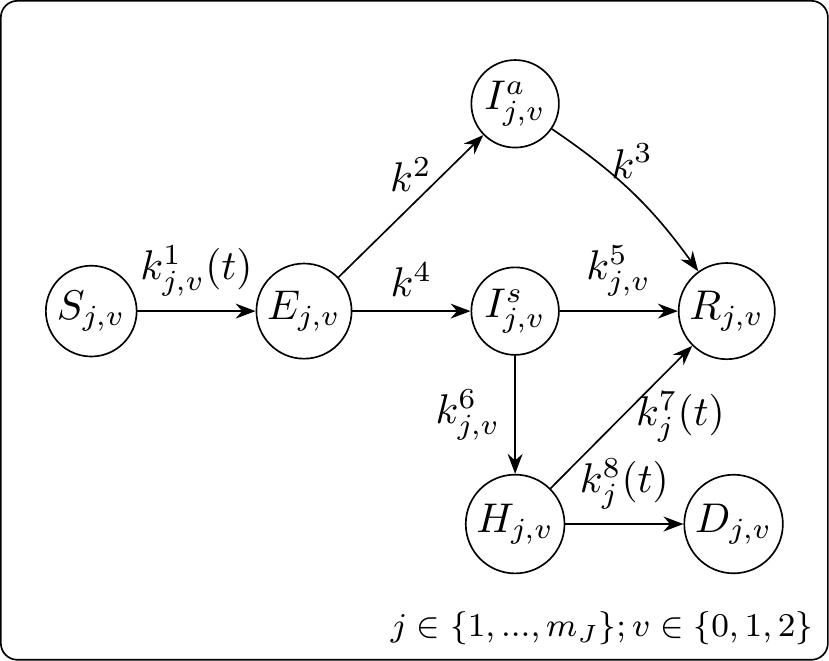
\includegraphics{README_files/figure-latex/statetransitions-1.png}
\caption{\label{fig:statetransitions}Disease state transitions. \(S\): susceptible. \(E\): exposed. \(I^{a}\): asymptomatic infectious. \(I^{s}\): symptomatic infectious. \(H\): hospitalised. \(R\): recovered. \(D\): died. \(j\): stratum. \(v\): vaccination status.}
\end{figure}

\end{fignos:no-prefix-figure-caption}

Possible transitions between disease states are shown in Figure \ref{fig:statetransitions}. Transition rates are functions of time \(t\), vaccination status \(v\), and group identity \(j\) (where the groups are the 45 sectors and the four age groups).

The rate of infection of susceptible individuals, \(`k^{1}_{j,v}(t)`\), is defined as

\begin{equation}
k_{j,v}^{1}(t) = \eta_{v}^{E}\rho(t)\beta\sum_{h=1}^{m_J}M_{j,h}(x) I_h(t)
\label{eq:infection}
\end{equation}

with \(m_J=49\) strata and

\begin{verbatim}
 I_h(t)=\sum_{v=0}^{m_V}\left(\epsilon (1-p^3(t))I_{h,v}^{a}(t)+(1-p^4(t))I_{h,v}^{s}(t)\right). 
\end{verbatim}

Here, \(`\eta^{E}_{v}`\) is the relative probability to be infected given vaccine status \(v\); \(\rho(t)\) is the time-dependent modifier of the rate of infection, \(\beta\), which captures the impact of social distancing; \(M(x)\) is the contact matrix between groups and depends on the economic configuration \(x\); \(\epsilon\) is the reduction in infectiousness from asymptomatic relative to symptomatic individuals; \(p^3\) and \(p^4\) are the proportions of asymptomatic and symptomatic infectiousness averted, respectively, due to self isolating; and \(I_{h,\cdot}^{\cdot}\) is the number of infectious asymptomatic (\(I_{h,\cdot}^{a}\)) and symptomatic (\(I_{h,\cdot}^{s}\)) people who are unvaccinated (\(I_{h,v=0}^{\cdot}\)), vaccinated with the BPSV (\(I_{h,v=1}^{\cdot}\)), or vaccinated with the specific vaccine (\(I_{h,v=2}^{\cdot}\)) in stratum \(h\).

\begin{verbatim}
 k^2 = \big(1-p^{I^S}\big)/T^{E:I} 
\end{verbatim}

is the rate to asymptomatic infectiousness, where \(p^{I^S}\) is the probability to become symptomatic given infection, and \(T^{E:I}\) is the expected duration of the latent period before the onset of infectiousness;

\begin{verbatim}
 k^3 = 1/T^{I^a:R}  
\end{verbatim}

is the rate of recovery from asymptomatic infection;

\begin{verbatim}
 k^4 = p^{I^S}/ T^{E:I}; 
\end{verbatim}

is the rate of symptom onset;

\begin{verbatim}
k^{5}_{j,v} =  \big(1-p^H_{j,v}\big) / T_{j,v}^{I^s}
\end{verbatim}

is the rate of recovery from symptomatic infection, where \(p^H_{j,v}\) is the probability to be hospitalised given symptomatic infection, and \(T_{j,v}^{I^s} = p^H_{j,v}T^{I^s:H} + (1-p^H_{j,v})T^{I^s:R}\) is the expected time to be in compartment \(I^s\): \(T^{I^s:H}\) is the expected duration before hospitalisation and \(T^{I^s:R}\) is the expected duration before recovery.

\begin{verbatim}
p^H_{j,v}=\eta^{H}_{v}\tilde{p}^{H}_{j}
\end{verbatim}

is the baseline probability to be hospitalised (\(`\tilde{p}^{H}_{j}`\)) adjusted by the vaccine effect protecting against hospitalisation (\(`\eta^{H}_{v}`\)). Then

\begin{verbatim}
k^{6}_{j,v} = p^H_{j,v}/T_{j,v}^{I^s}
\end{verbatim}

is the rate of hospitalisation following symptomatic infection.

\begin{verbatim}
k^{7}_{j}(t) = (1-p^{D}_{j}(t)) / T_j^{H}(t)
\end{verbatim}

is the rate of recovery of hospitalised patients, where \(`p^{D}_{j}(t)=\tilde{p}^{D}_{j}f_H(t)`\) is the baseline probability to die given hospitalisation, adjusted by a factor encoding the increase in fatality rate as hospital occupancy increases:

\begin{verbatim}
f_H(t)=\max\{1,1+1.87(H_{\text{tot}}(t)-H_{\text{max}})/H_{\text{max}}\},
\end{verbatim}

\begin{verbatim}
H_{\text{tot}}(t) = \sum_{v=0}^{m_V}\sum_{j=1}^{m_J} H_{j,v}(t).
\end{verbatim}

\[T_j^{H}(t) = p_j^{D}(t)T^{H:D} + (1-p_{j}^{D}(t))T^{H:R}\]

is the expected time to be in compartment \(H\): \(T^{H:D}\) is the expected duration before death and \(T^{H:R}\) is the expected duration before recovery. Finally,

\begin{verbatim}
k^{8}_{j}(t) = p^{D}_{j}(t)/T_j^{H}(t)
\end{verbatim}

is the rate of death following hospitalisation.

\hypertarget{vaccination-state-transitions}{%
\subsection{Vaccination state transitions}\label{vaccination-state-transitions}}

In our model, \(v=0\) refers to unvaccinated people, \(v=1\) to people who have received a full schedule of BPSV, and \(v=2\) to people who have received a full schedule of the specific vaccine. How we model transitions between vaccination states is shown in Figure \ref{fig:vaccinetransitions}.

\(`k^{10,c_1}_{j,v=0}(t)`\) represents the rates of BPSV vaccination of unvaccinated susceptible and recovered people, and \(`k^{10,c_2}_{j,v=1}(t)`\) represents the rates of vaccinating BPSV-vaccinated susceptible and recovered people. \(`k^{10,c_2}_{j,v=0}(t)`\) represents the rates of vaccinating people directly with the specific vaccine. Put more succintly, \(`k^{10,c_u}_{j,v}(t)`\) is the rate to go from vaccine state \(v\) to \(u\). \(k^9=1/T^c\) is the rate of seroconversion to vaccine-induced immunity, and \(`k^{12}_{j}(t)=k^{1}_{j,v=0}(t)`\) and \(`k^{19}_{j}(t)=k^{1}_{j,v=1}(t)`\) are the rates of infection of just-vaccinated people, which returns them to the epidemiological pathway of the lower vaccination level.

\begin{fignos:no-prefix-figure-caption}

\begin{figure}
\centering
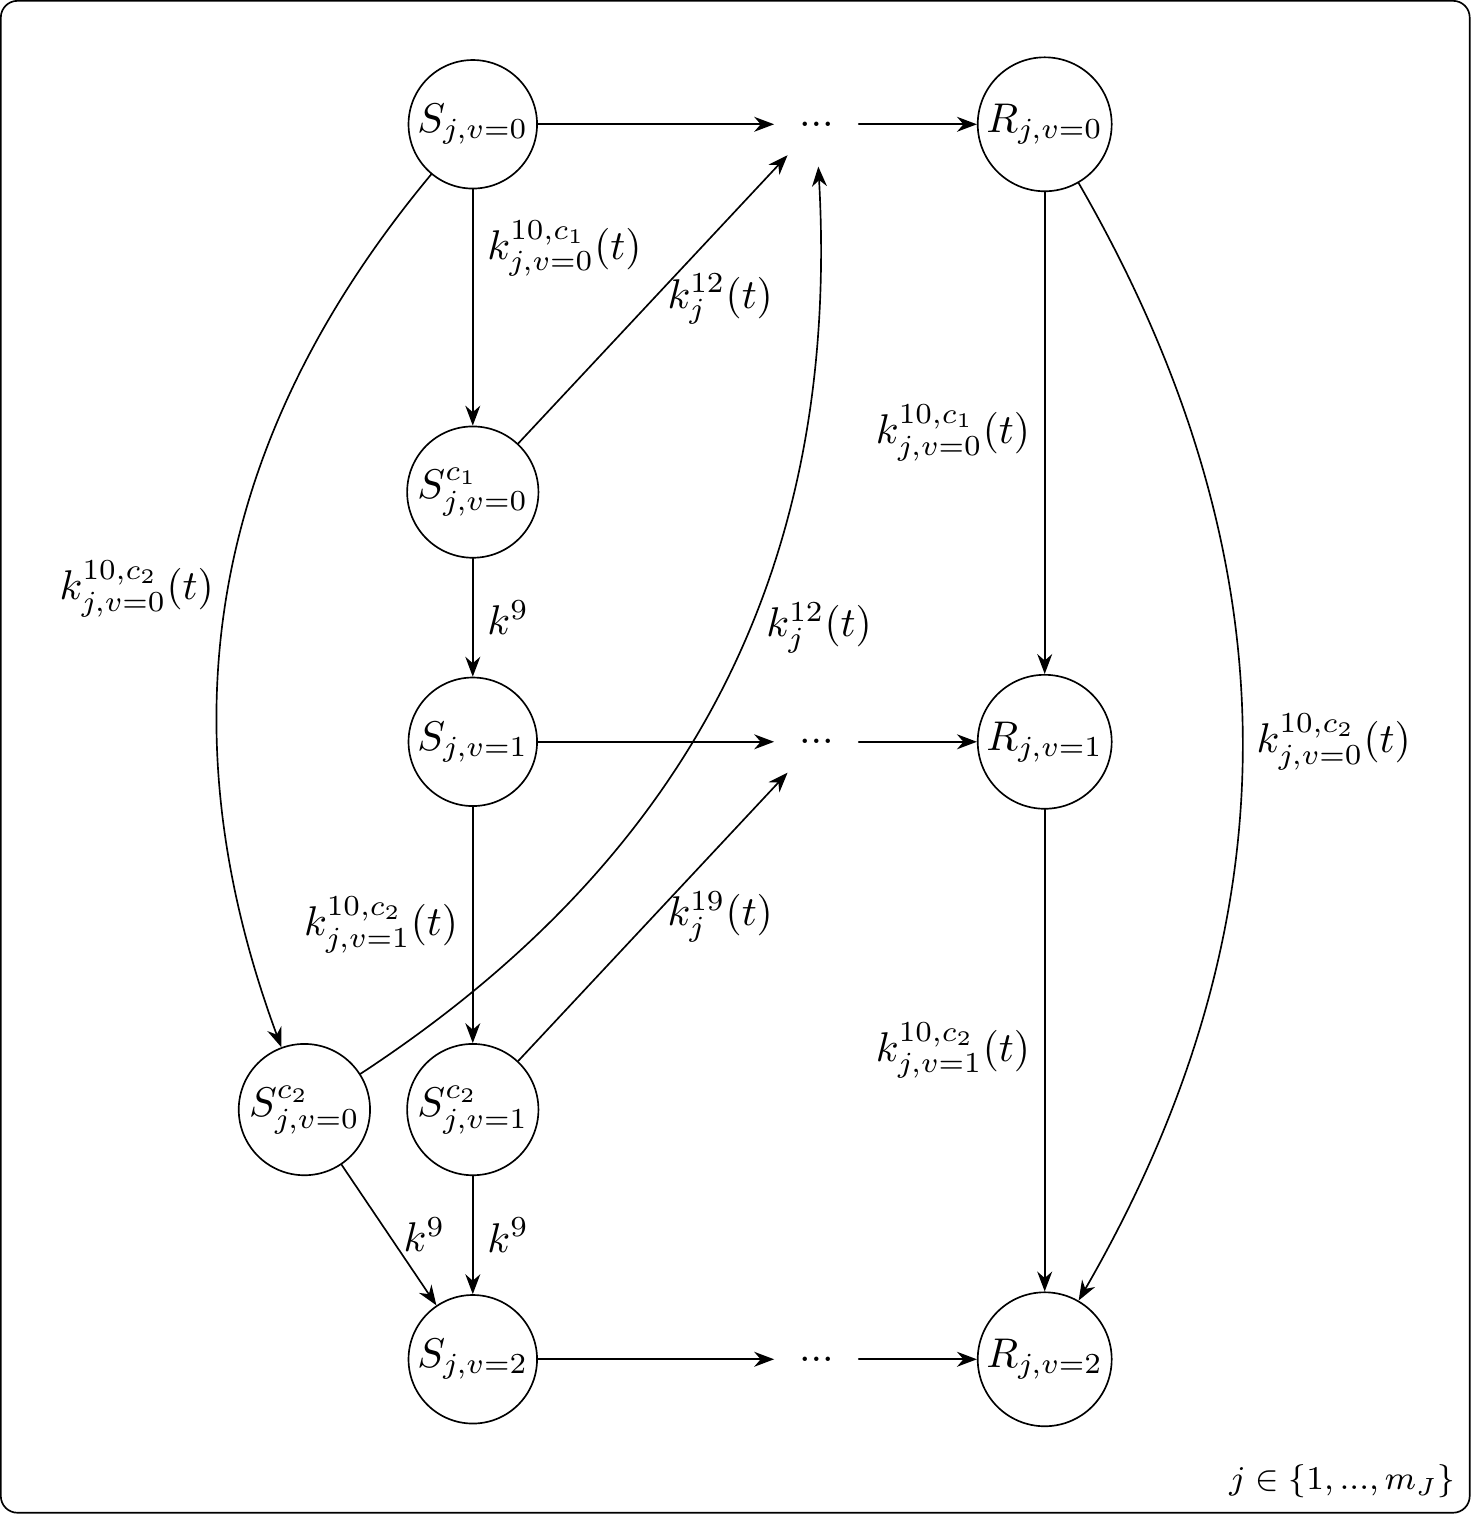
\includegraphics{README_files/figure-latex/vaccinetransitions-1.png}
\caption{\label{fig:vaccinetransitions}Vaccine state transitions. \(S\): susceptible. \(S^{c_u}, u\in\{1,2\}\): recently vaccinated but has not yet seroconverted (i.e.~is not protected by most recent vaccination). \(R\): recovered. \(j\): stratum. \(v\): initial vaccination status. \(u\): final vaccination status.}
\end{figure}

\end{fignos:no-prefix-figure-caption}

\hypertarget{contact-rates}{%
\subsection{Contact rates}\label{contact-rates}}

The configuration \(x\) and the proportion of workers working from home \(q\) determine the scaling of exposure to infection between different groups for different reasons:

\begin{itemize}
\tightlist
\item
  Worker absence due to sector closure
\item
  Worker absence due to working from home
\item
  Student absence due to school closure
\item
  Customer absence due to sector closure: impact on workers
\item
  Customer absence due to sector closure: impact on customers
\end{itemize}

We approach this differently from (Haw et al. 2022). Instead of contact matrices from (Prem et al. 2021), we use those from (Walker et al. 2020). Instead of work contacts from (Béraud et al. 2015), we use those from (Jarvis et al. 2023). (Haw et al. 2022) modelled closures using a combination of moving workers between sector compartments and a non-working compartment, and scaling of contacts. Here, we only use contacts to model closures, and do not move workers out of their compartments. An advantage of this is that workers within sectors retain their infection histories.

We construct contact matrix \(M(x)\) as the sum of three matrices: \(M^{\text{com}}(x)\) (community contacts), \(M^{\text{CW}}(x)\) (community-to-worker contacts), and \(M^{\text{WC}}(x)\) (worker-to-community contacts). We construct peacetime matrices (\(x=\textbf{1}\)) beginning with a ``target matrix,'' which the three matrices should add up to, which is taken from (Walker et al. 2020). By sampling relevant values, we decompose the whole matrix into its component parts. To incorporate closures, each matrix is transformed independently, before they are all added together again.

Matrix \(M(\textbf{1})\) is estimated using as a basis a contact matrix from (Walker et al. 2020). These are 16-by-16 matrices, \(\tilde{M}\), for five-year age bands \(a\) up to age group 75+. We map the matrix to a four-by-four matrix \(\hat{M}\) corresponding to the four age groups \(g\) used in the DAEDALUS model, using population sizes \(\tilde{N}_a\):

\begin{verbatim}
\hat{M}_{gg'} = \frac{\sum_{a\in g}\tilde{N}_{a}\sum_{a'\in g'}\tilde{M}_{a,a'}}{\sum_{a\in g}\tilde{N}_{a}},
\end{verbatim}

and \(\hat{N}_g\) to represent the population sizes of the DAEDALUS age groups,

\begin{verbatim}
\hat{N}_g=\sum_{a\in g}\tilde{N}_a.
\end{verbatim}

We get to the matrix \(M(\textbf{1})\) by broadcasting the four-by-four matrix to the 49-by-49 one. Contacts from all groups \(j\) to working groups \(h\) depend on the age group of the group (\(`g(j)`\)), and the fraction of the age-population represented in group \(h\), where \(N_{h}\) is the number of people in group \(h\):

\begin{verbatim}
M_{j,h}(\textbf{1}) = \hat{M}_{g(j),g(h)}\frac{N_{h}}{\hat{N}_{g(h)}}
\end{verbatim}

for \(j\) and \(h\) including all groups (working and non-working). Each group \(j\) contains people that belong to only one age group \(g\). We refer to the age group of the people in group \(j\) as \(g(j)\). Then \(\hat{N}_{g(h)}\) is the number of people in the age group of group \(h\), so \(`\hat{N}_{g(h)}=N_{h}`\) for age groups 0 to 4, 5 to 19 and 65+, and \(`\hat{N}_{g(h)}=\sum_{h\in\{1,...,m_S,m_S+3\}}N_{h}`\) for age group 20 to 64.

In setting up a country, we sample values for \(\tilde{M}\) (from which we get \(`M(\textbf{1})`\)). At the same time, we sample the proportion of contacts that come from workplaces, and workplace-related contacts. From these, we get \(M^{\text{CW}}(\textbf{1})\), constructing the matrices and normalising.

Consumer-to-worker contacts (matrix \(M^{\text{CW}}\)) describe contacts experienced by workers from consumers per sector. Note that \(`M^{\text{CW}}_{j,h}(\textbf{1})=0`\) for \(j>m_S\). Matrix \(M^{\text{WC}}(\textbf{1})\) is the complement of matrix \(M^{\text{CW}}(\textbf{1})\), computed by multiplying through by population, transposing, and dividing again by population.

With \(M(\textbf{1})\), \(M^{\text{CW}}(\textbf{1})\) and \(M^{\text{WC}}(\textbf{1})\), we learn \(M^{\text{com}}(\textbf{1})\).

\(M^{\text{com}}(\textbf{1})\) is decomposed into its constituent parts, representing intra- and inter-household interactions (home), school interactions (sch) and hospitality interactions (CC):

\begin{verbatim}
M^{\text{com}}(\textbf{1})=M^{\text{home}} + M^{\text{sch}}(\textbf{1}) + M^{\text{CC}}(\textbf{1}) 
\end{verbatim}

Values for \(M^{\text{sch}}(\textbf{1})\) come from sampled values representing the fractions of contacts that come from school. School contacts are estimated separately in two age groups (pre-school age: 0-\/--4 (Figure \ref{fig:school1frac}); school age: 5-\/--19 (Figure \ref{fig:school2frac})): \(M^{\text{sch}}(\textbf{1})\) has entries of zero for groups not in school, and values for 0 to 4 year olds and 5 to 19 year olds.

Finally, \(M^{\text{CC}}(\textbf{1})\) is sampled as a fraction of \(M^{\text{com}}(\textbf{1})- M^{\text{sch}}(\textbf{1})\) (Figure \ref{fig:hospfrac}), which leaves \(M^{\text{home}}\).

\begin{figure}
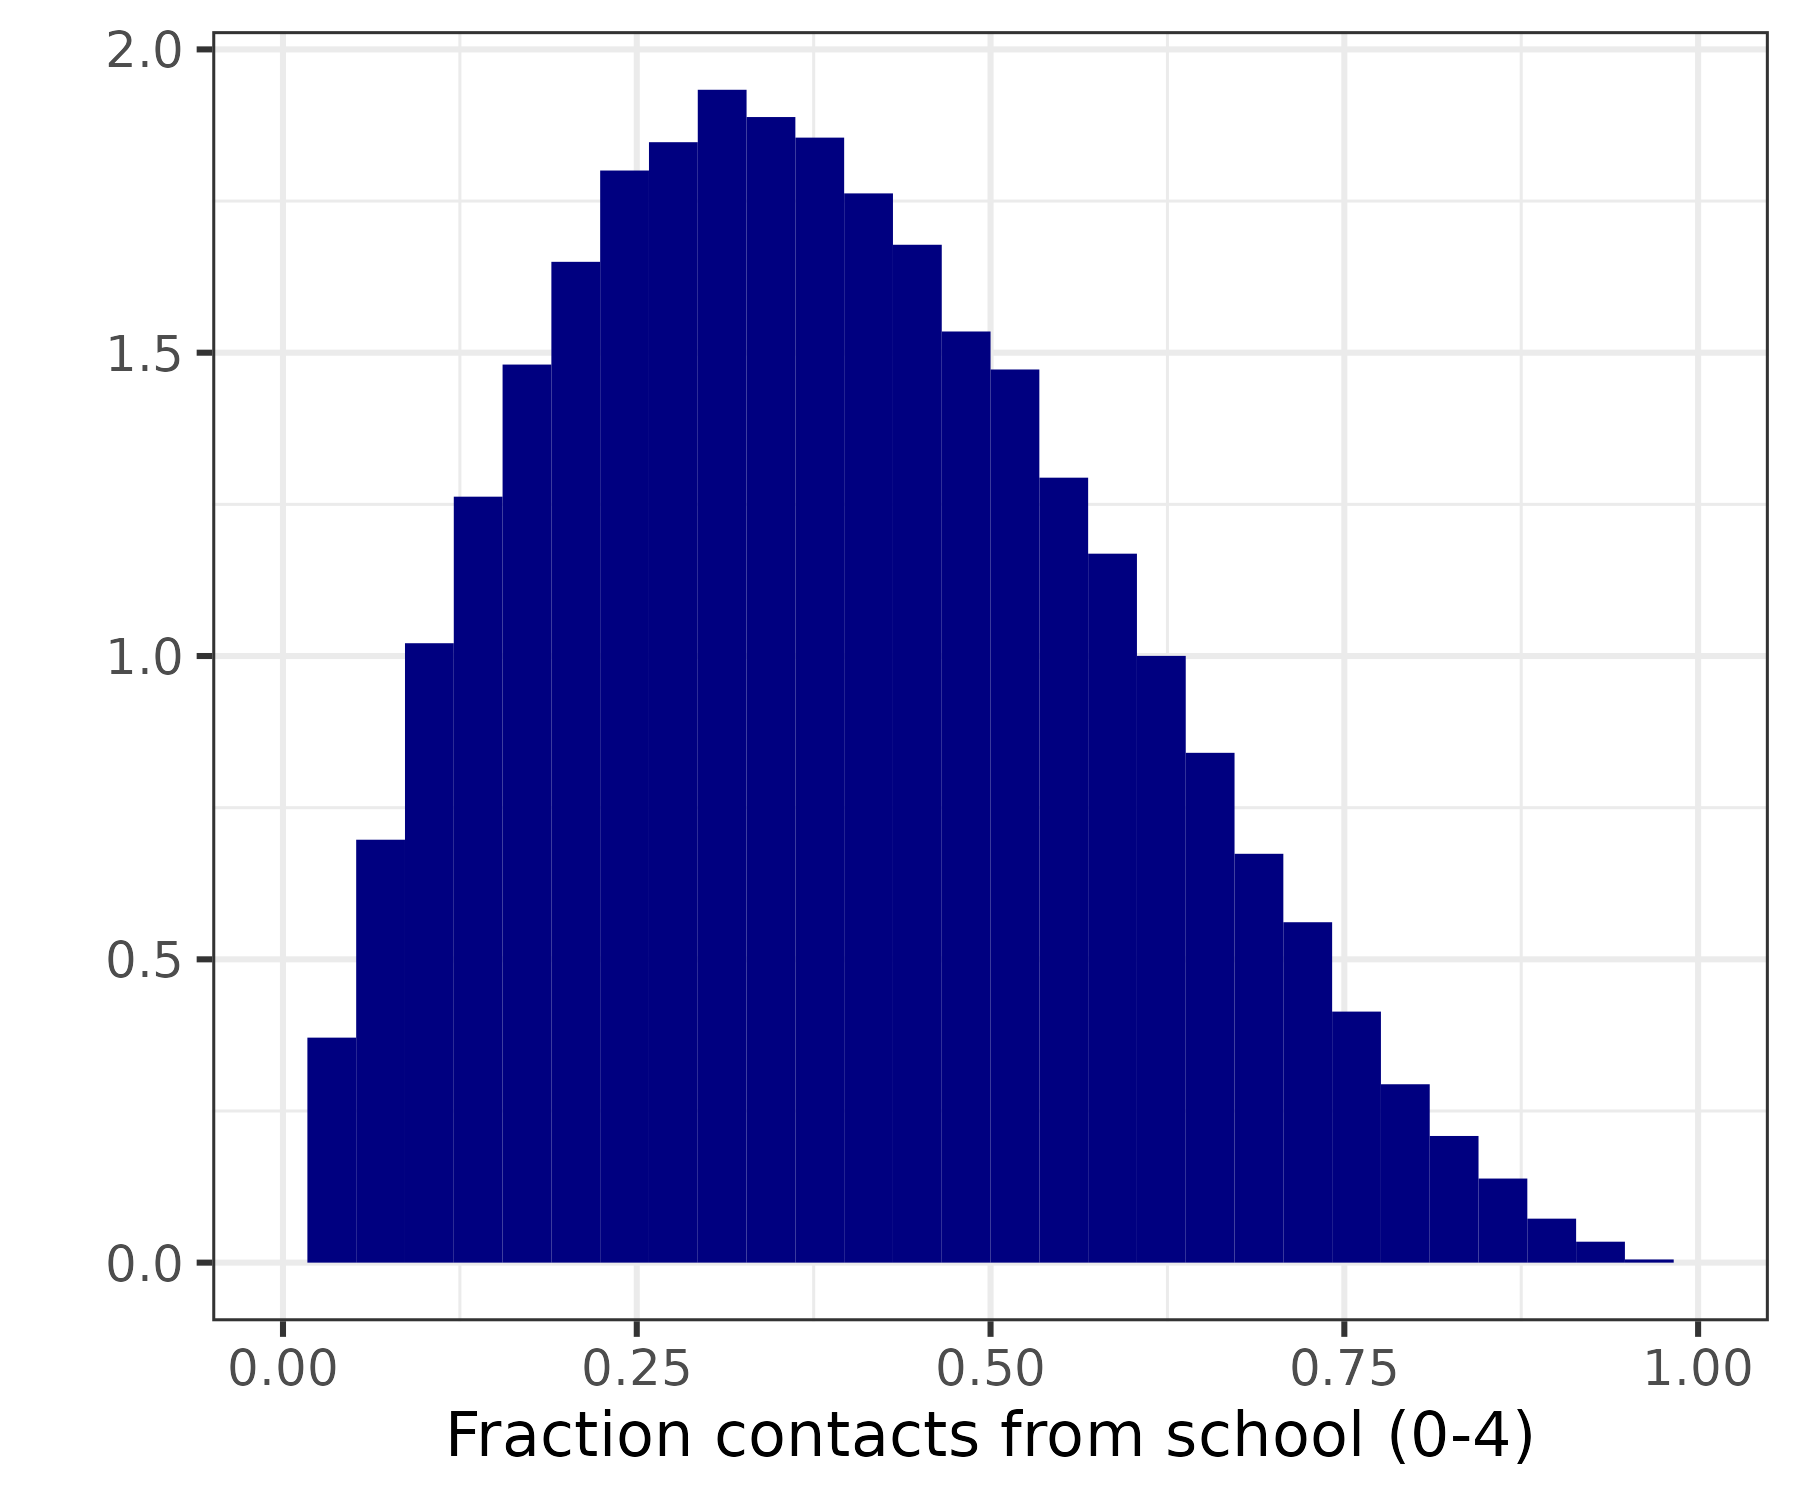
\includegraphics[width=25in]{README_files/figure-gfm/school1frac} \caption{Fraction of contacts made at school for ages 0 to 4.}\label{fig:school1frac}
\end{figure}

\begin{figure}
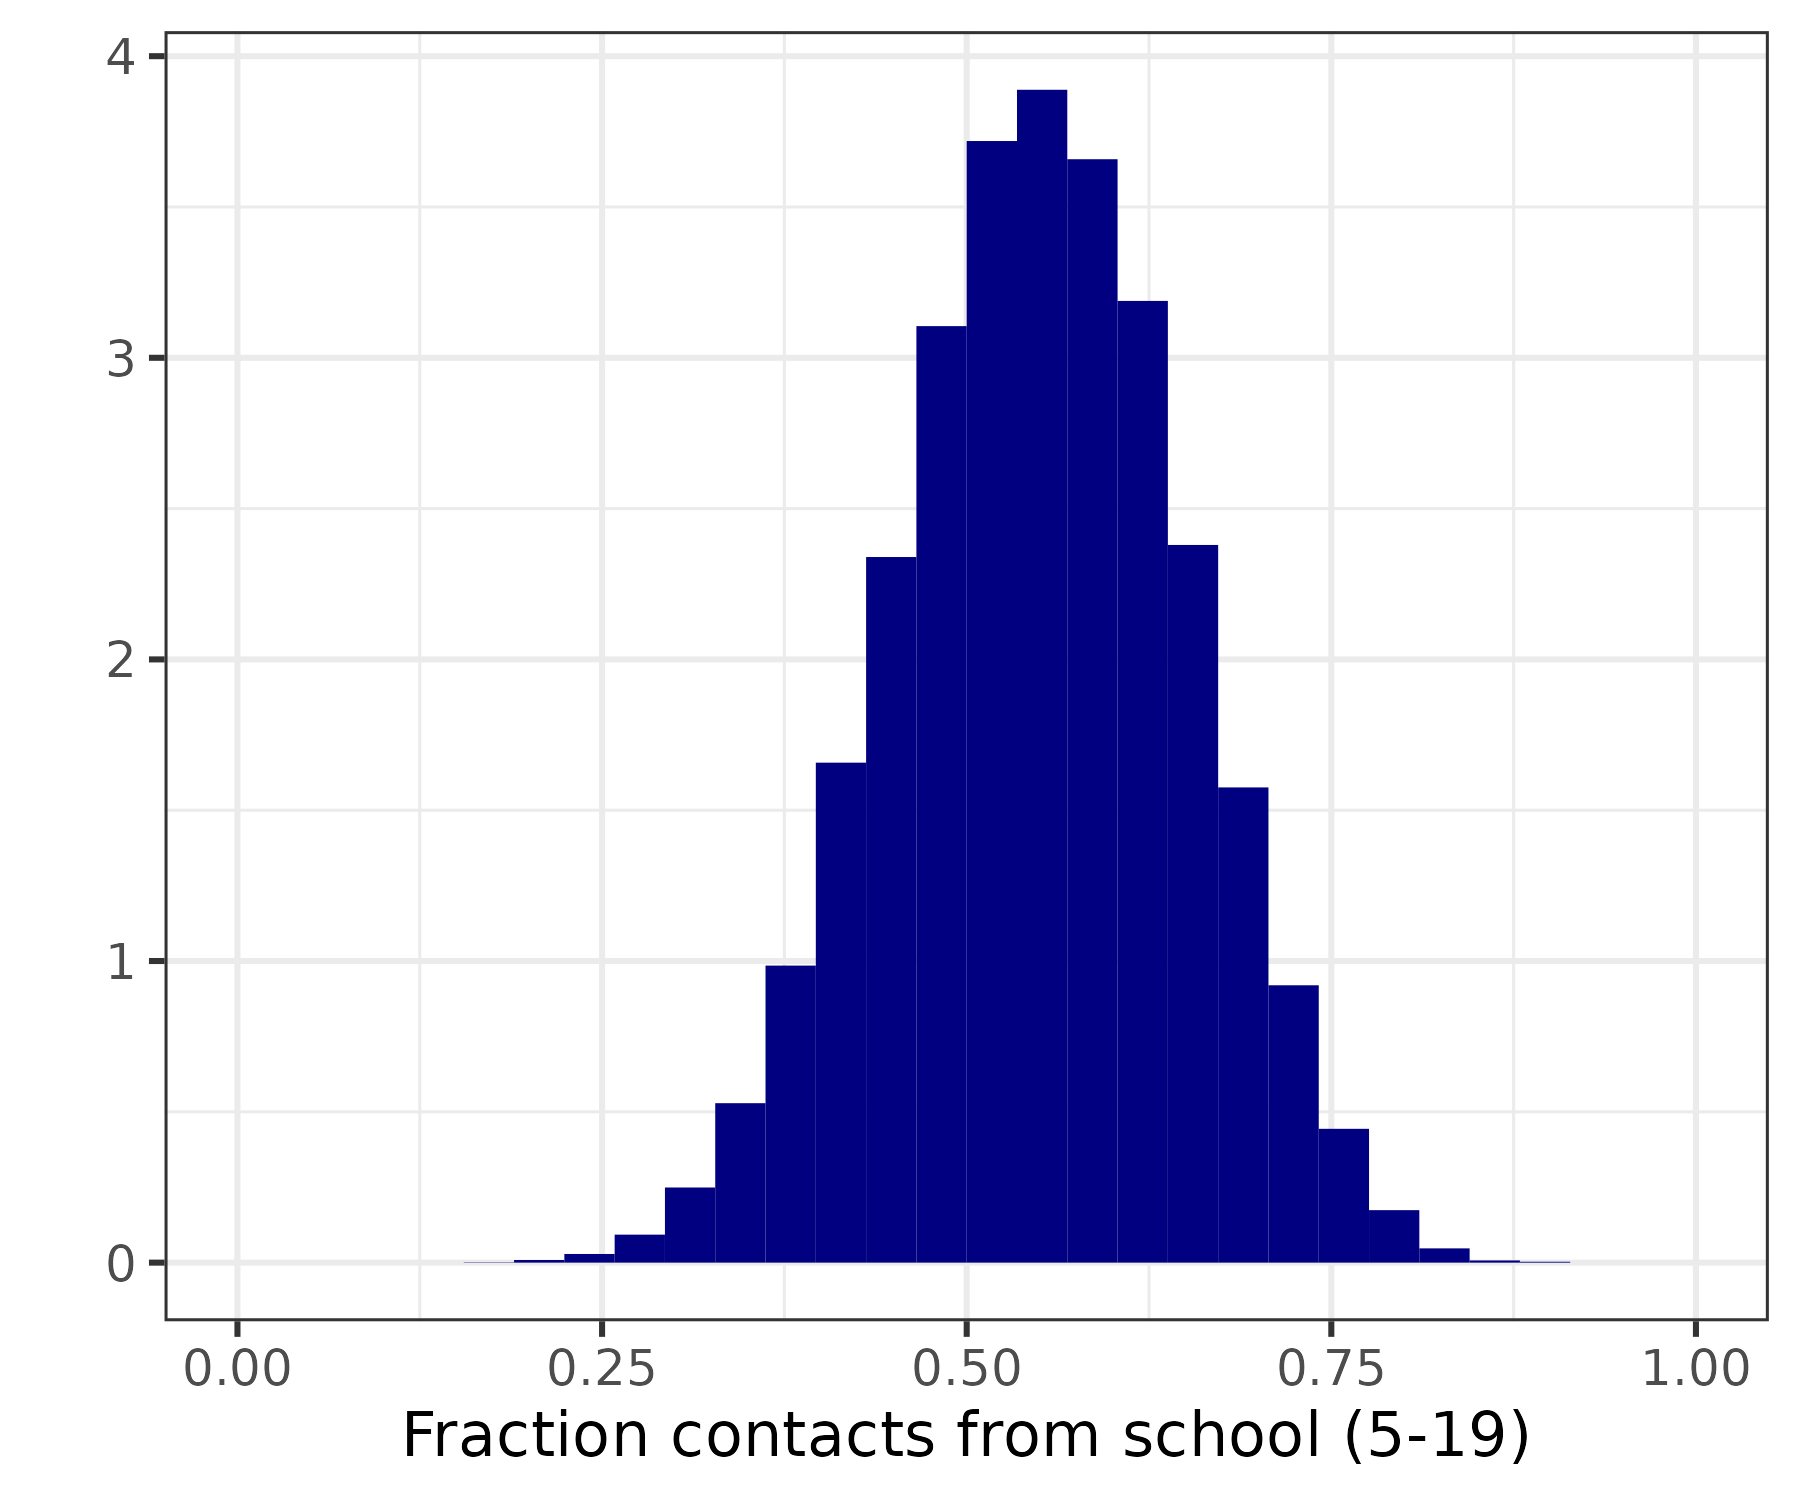
\includegraphics[width=25in]{README_files/figure-gfm/school2frac} \caption{Fraction of contacts made at school for ages 0 to 4.}\label{fig:school2frac}
\end{figure}

\begin{figure}
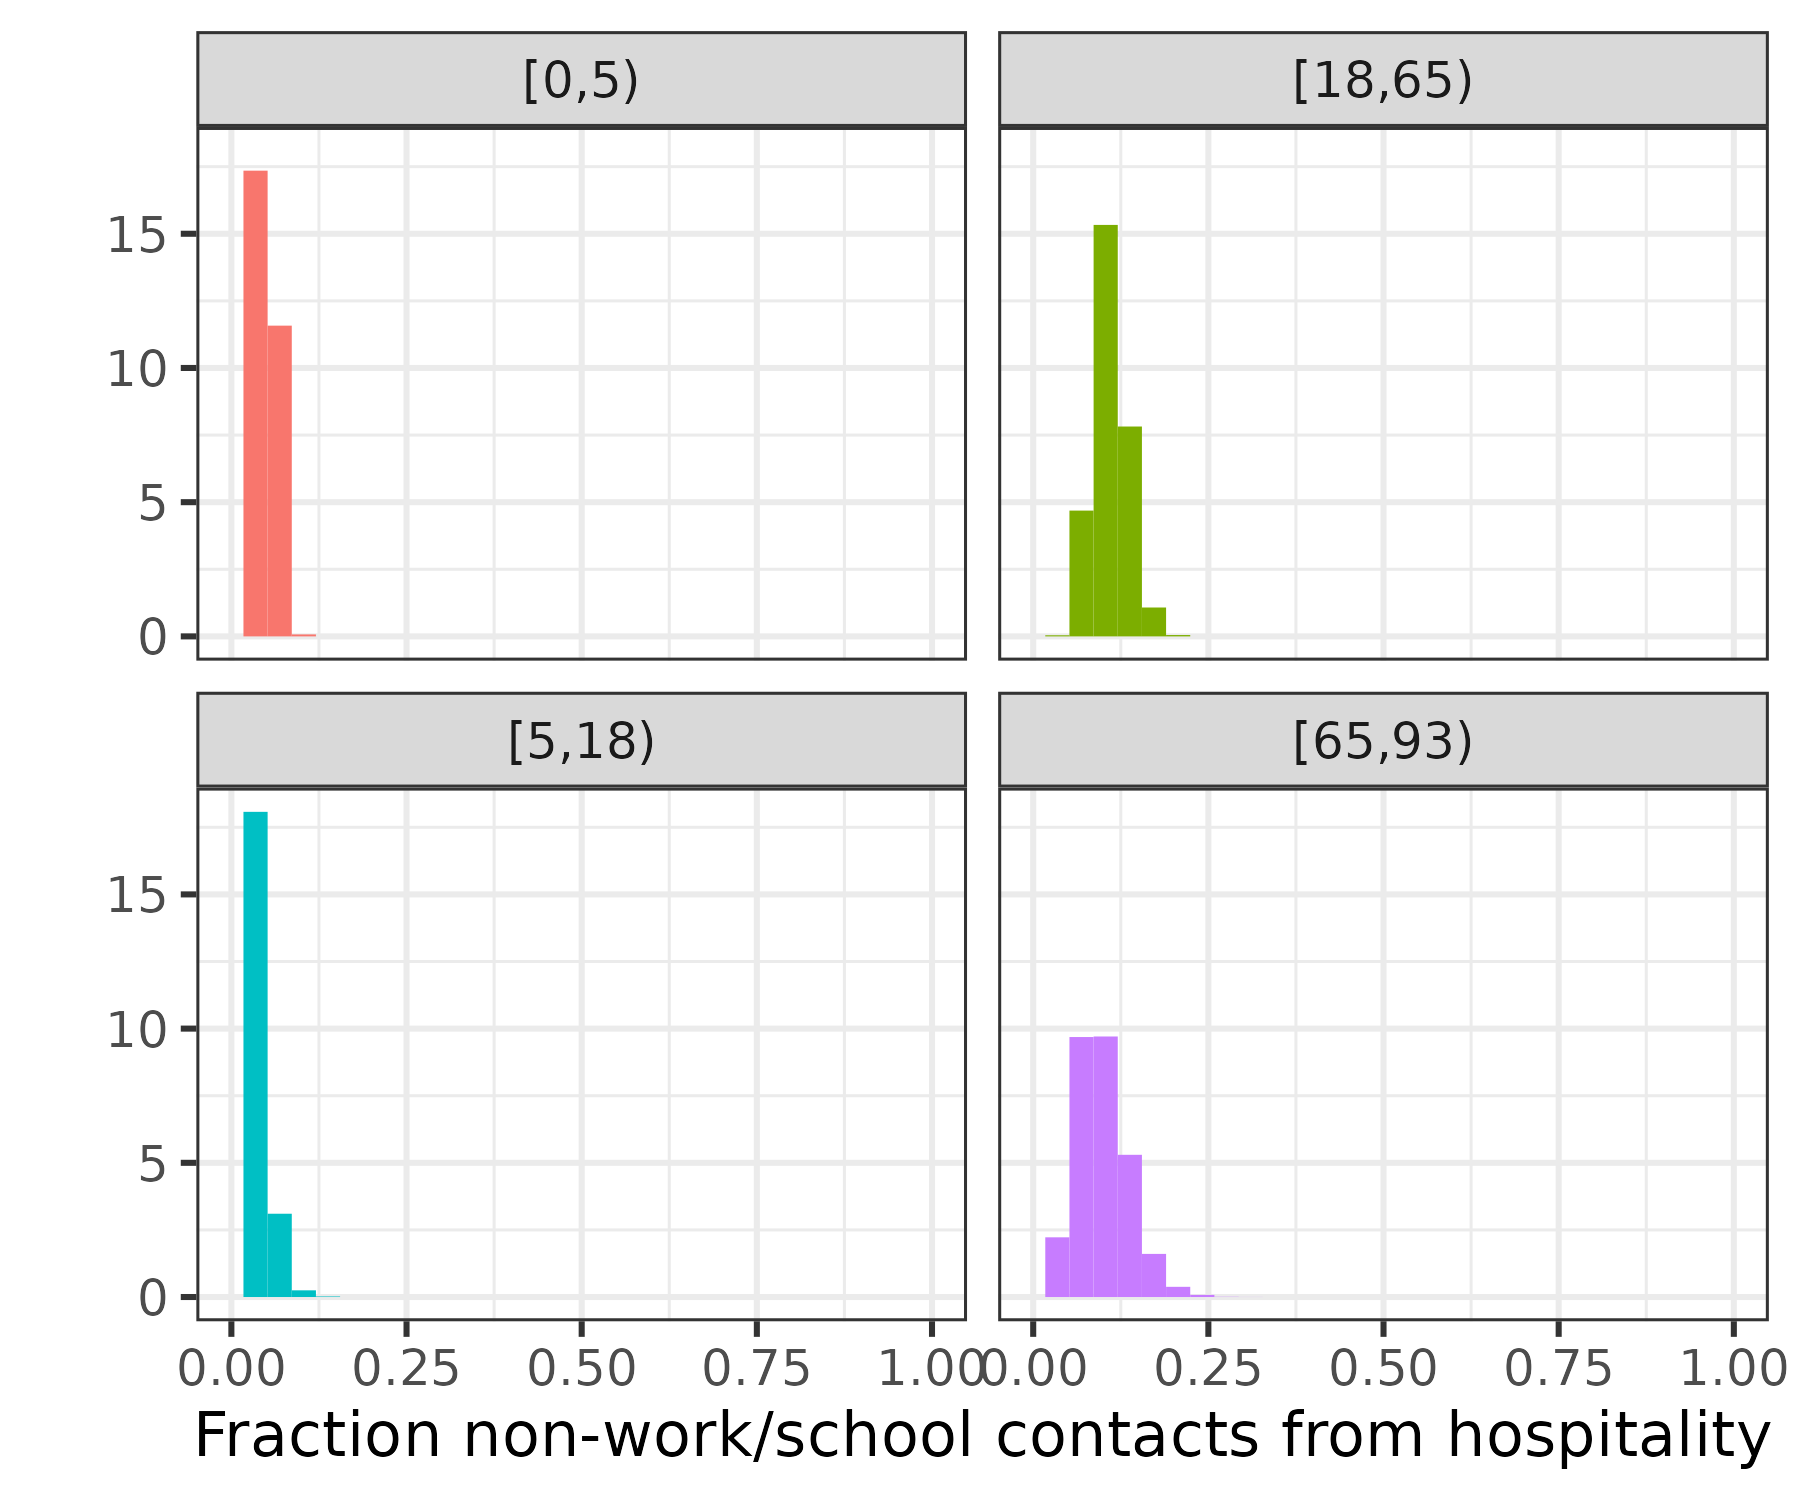
\includegraphics[width=25in]{README_files/figure-gfm/hospfrac} \caption{Fraction of non-school and non-work contacts made in hospitality settings, by age group.}\label{fig:hospfrac}
\end{figure}

\hypertarget{matrix-mtextcom-community-contacts}{%
\subsubsection{\texorpdfstring{Matrix \(M^{\text{com}}\): community contacts}{Matrix M\^{}\{\textbackslash text\{com\}\}: community contacts}}\label{matrix-mtextcom-community-contacts}}

We construct \(M^{\text{com}}(x)\) from its constituent parts, representing intra- and inter-household interactions (home), school interactions (sch) and hospitality interactions (CC):

\begin{verbatim}
M^{\text{com}}(x)=M^{\text{home}} + M^{\text{sch}}(x) + M^{\text{CC}}(x).
\end{verbatim}

School contacts under \(x\) are the peacetime values scaled by the extent of closure. \(x_{\text{ed}}\) is the extent to which schools are open, so that the number of contacts per person scales superlinearly with school closure.

\begin{equation}
M_{j,j}^{\text{sch}}(x)=x_{\text{ed}}^2M_{j,j}^{\text{sch}}(\textbf{1}).
\label{eq:school}
\end{equation}

Matrix \(M^{\text{CC}}(x)\) gives the contacts made in the hospitality sector:

\begin{equation}
M^{\text{CC}}(x) = (p^{27})^2M^{\text{CC}}(\textbf{1})
\label{eq:hosp}
\end{equation}

The value \(p^{27}\) is the workforce-weighted average extent to which the hospitality sectors are open, so that the number of contacts per person scales superlinearly according to closure:

\begin{verbatim}
p^{27} = \frac{\sum_jx_{j}N_j}{\sum_jN_j}
\end{verbatim}

where we sum over only the hospitality sectors.

\hypertarget{matrix-mtextcw-consumer-to-worker-contacts}{%
\subsubsection{\texorpdfstring{Matrix \(M^{\text{CW}}\): Consumer-to-worker contacts}{Matrix M\^{}\{\textbackslash text\{CW\}\}: Consumer-to-worker contacts}}\label{matrix-mtextcw-consumer-to-worker-contacts}}

\begin{equation}
M_{j,h}^{\text{CW}}(x) = (x_{j}(1-q_j))^2M_{j,h}^{\text{CW}}(\textbf{1}),
\label{eq:ctow}
\end{equation}

for \(h\in\{1,...,m_J\}\).

Here, there is superlinear scaling of \(M^{\text{CW}}_{j,h}(\textbf{1})\) with respect to working from home and with respect to sector closure, as both workers and members of the community are absent from the workplace as the sector moves online and becomes more closed.

\hypertarget{social-distancing}{%
\subsection{Social distancing}\label{social-distancing}}

We parametrise the effects of `social distancing' in the model using Google's mobility data (Figure \ref{fig:smoothmobility}). These changes in mobility were consequences of both government mandates and individual's choices. As we cannot separate the two, we consider a range of possibilities, based on the range of mobility changes observed for a given level of stringency (Figure \ref{fig:mobilitydrop}). In our model, the mandated economic configuration leads to a change in contacts. We associate the reduction in contacts, which translates as a relative reduction in transmission, with the reduction in mobility.

\begin{figure}
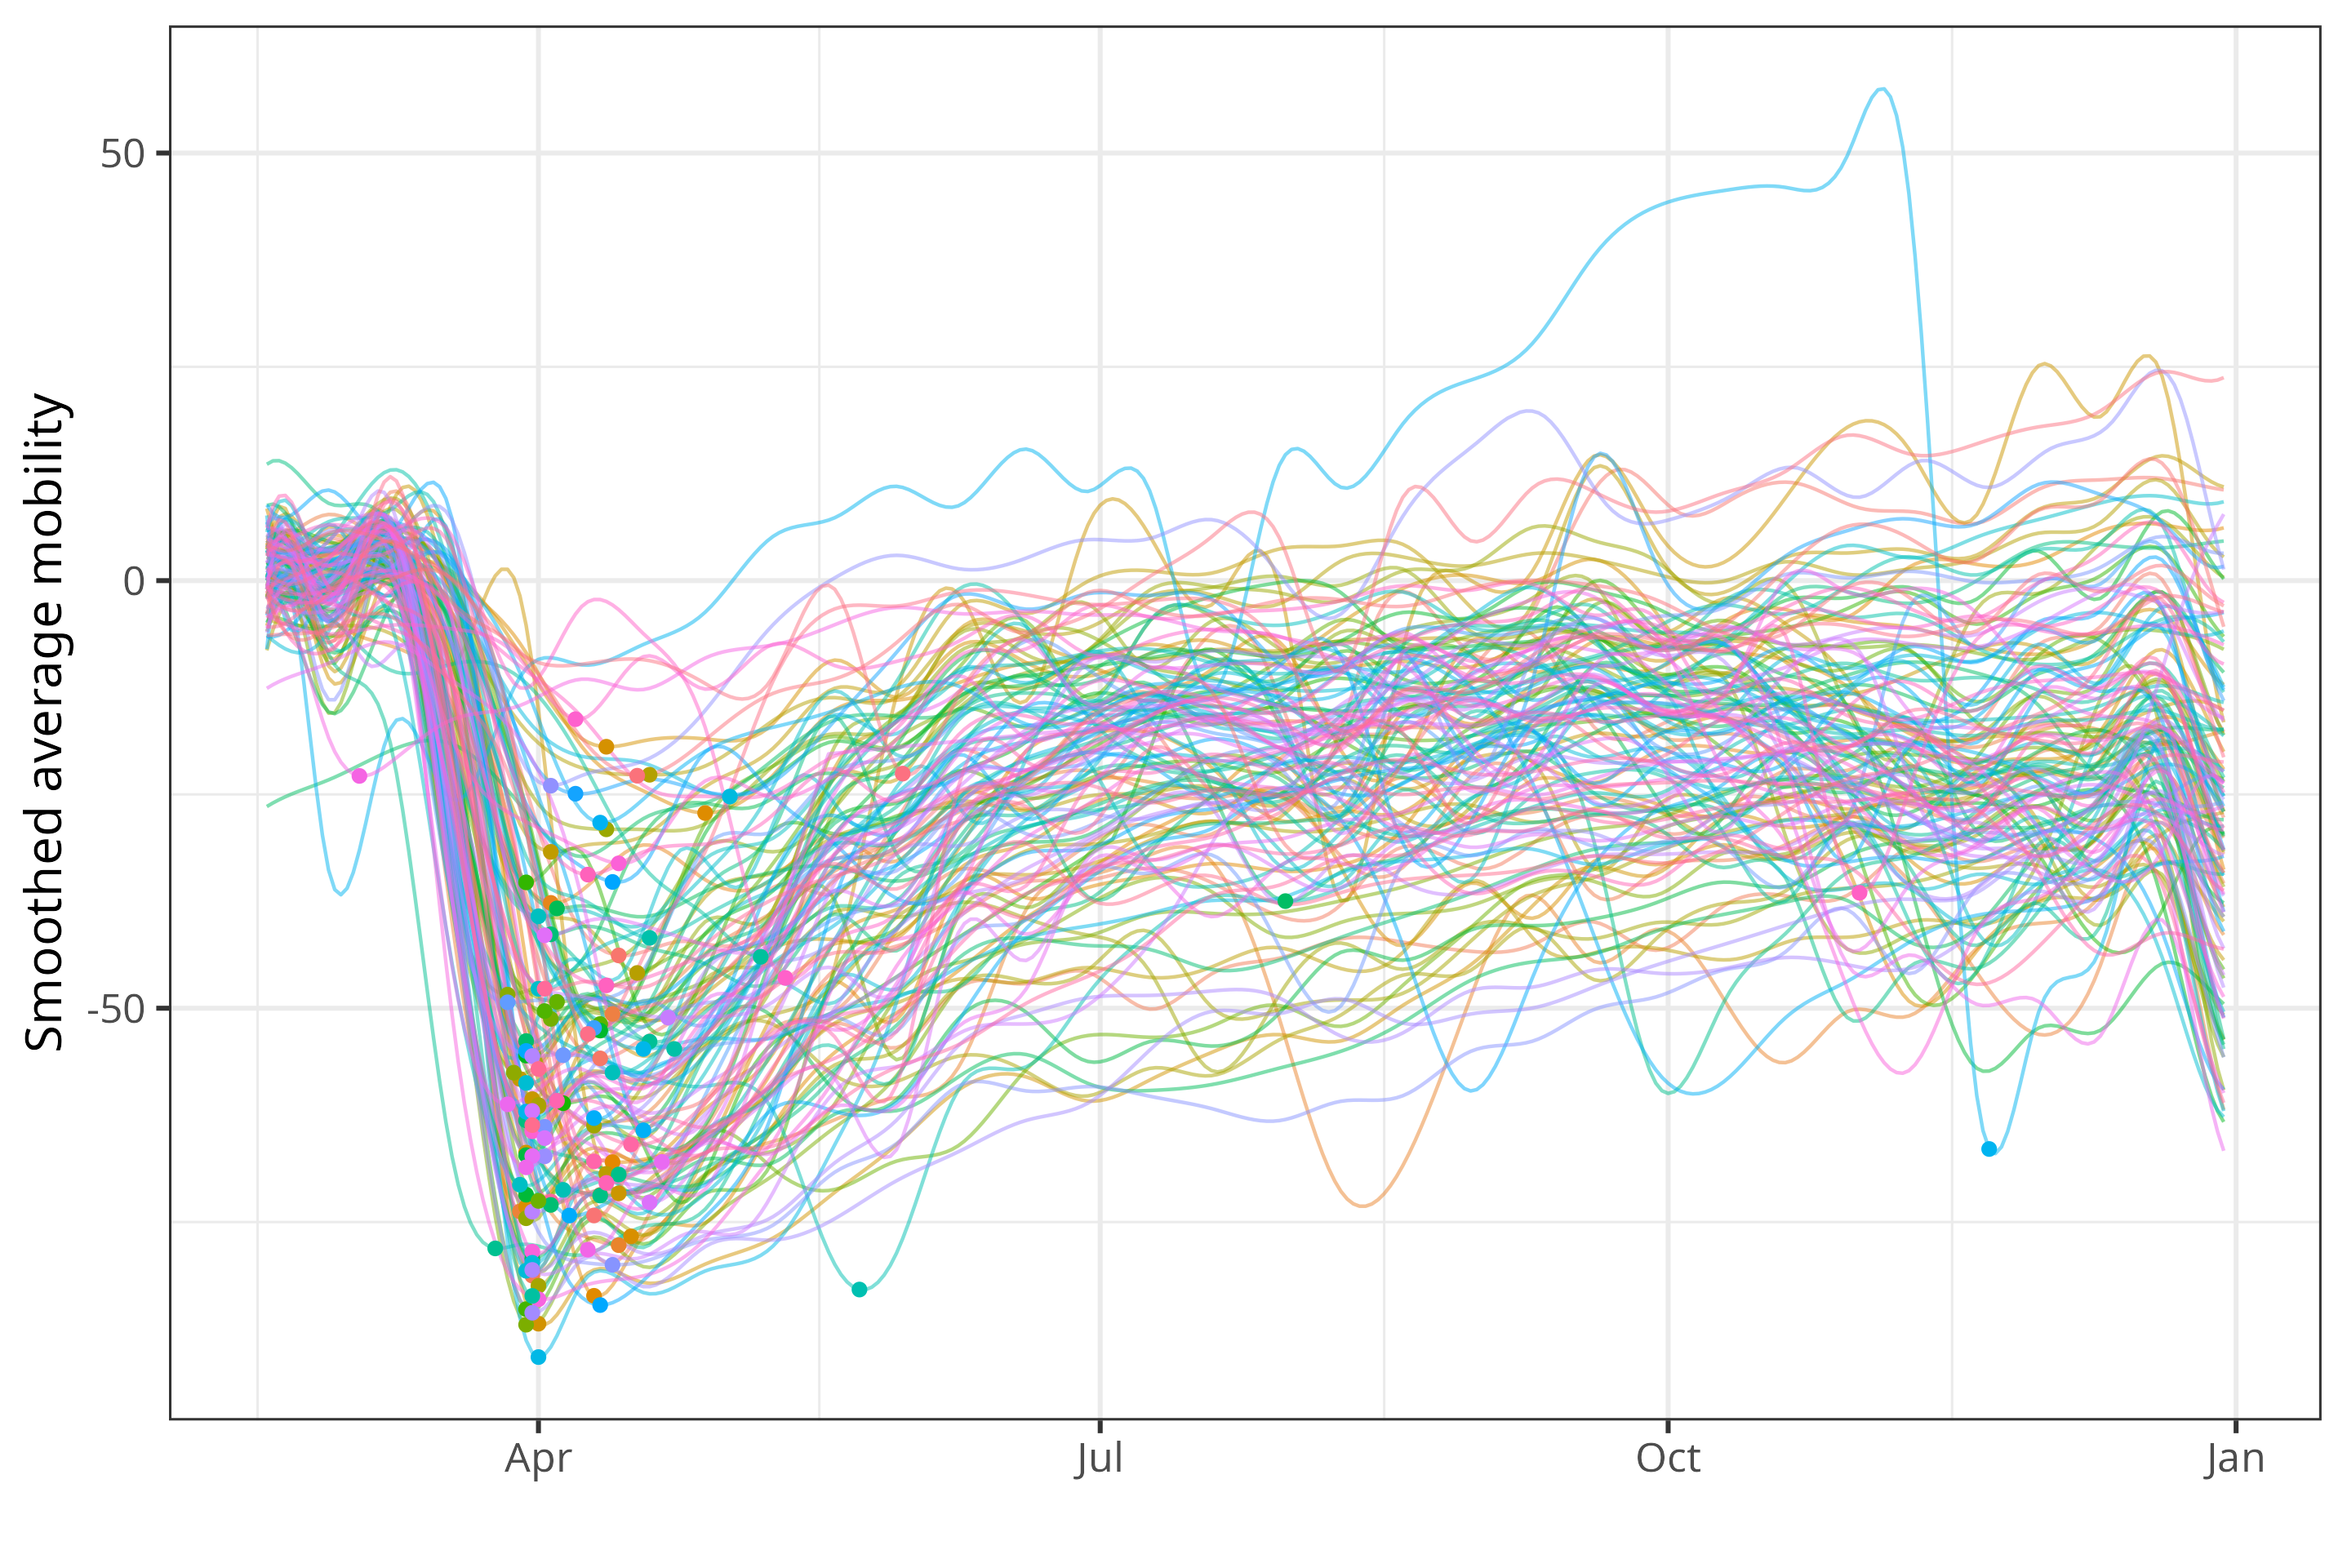
\includegraphics[width=39.01in]{README_files/figure-gfm/smoothmobility} \caption{Mobility trajectories in 2020 for all countries, with points showing the point at which the largest drop was observed. Trajectories are averaged over "Retail and recreation", "Transit stations" and "Workplaces" and smoothed with a spline of 80 knots.}\label{fig:smoothmobility}
\end{figure}

\begin{figure}
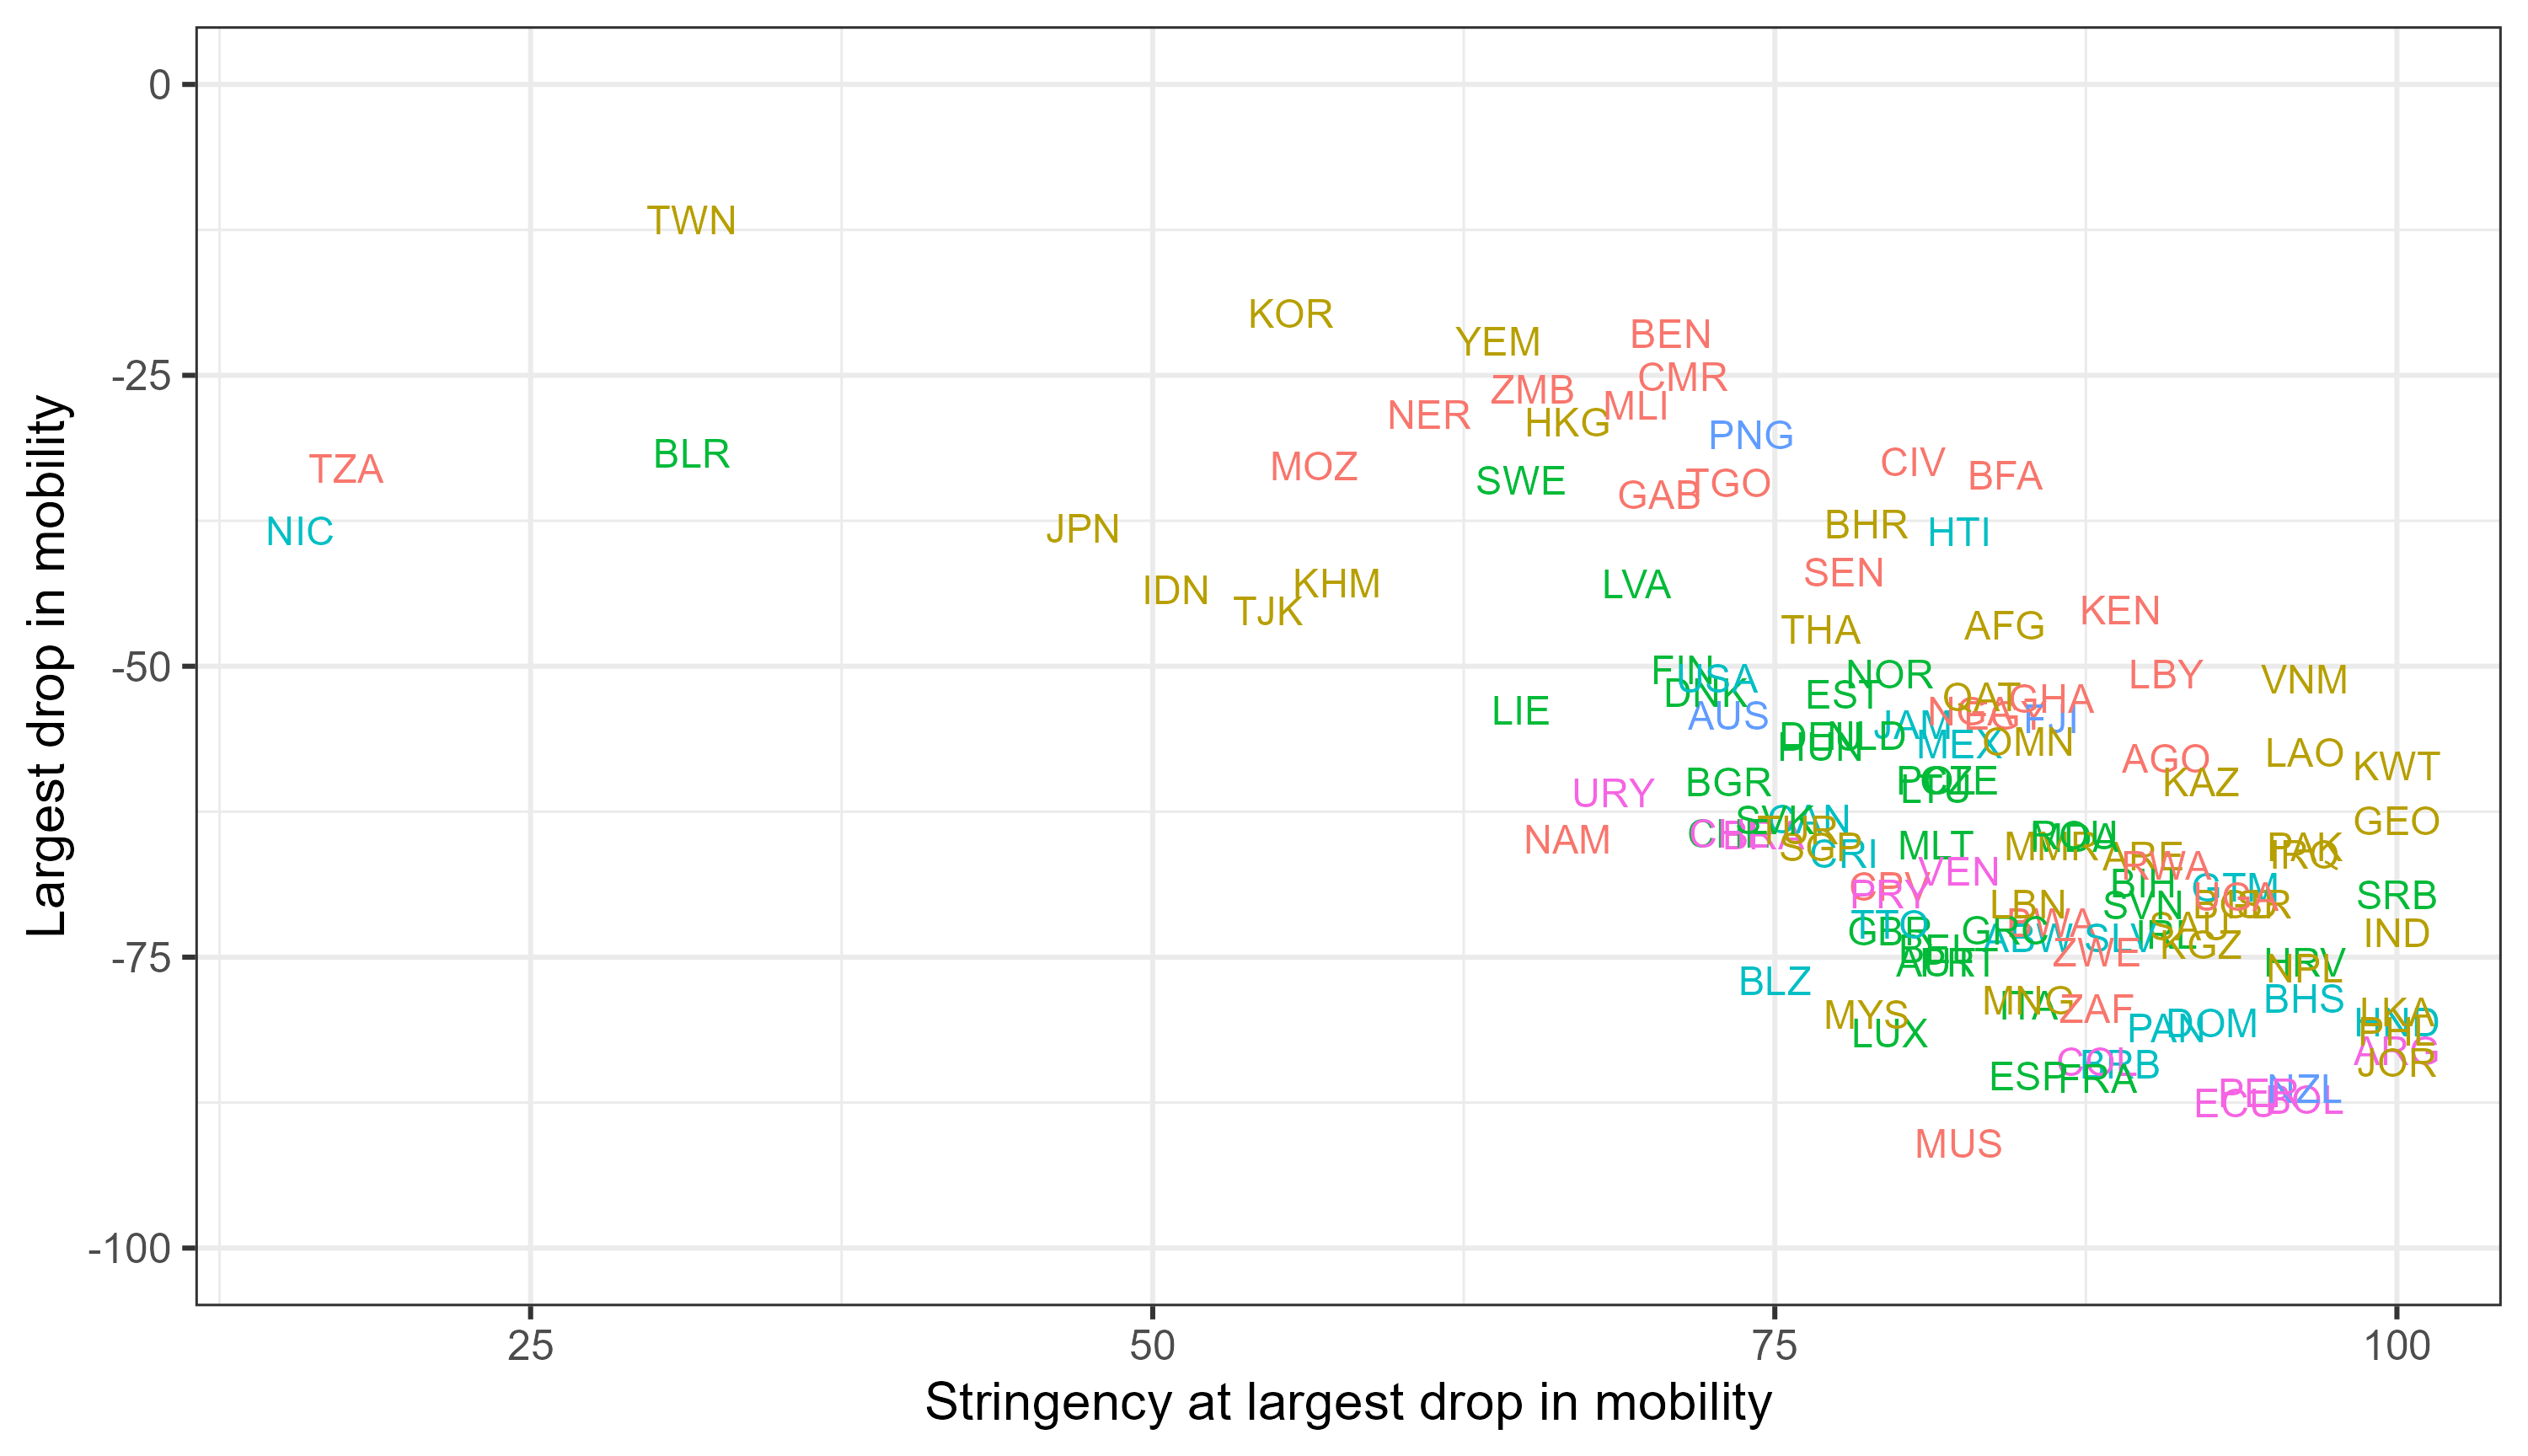
\includegraphics[width=41.67in]{README_files/figure-gfm/mobilitydrop} \caption{The largest drop in mobility plotted against the stringency on that date.}\label{fig:mobilitydrop}
\end{figure}

\begin{itemize}
\tightlist
\item
  We want to write mobility as a function of mandate and some epi outcome, e.g.~deaths: \(\rho(t) = (1-p^8)f(d(t),e(t)) + p^8\) where \(\rho(t)\) is mobility, \(d\) is deaths per million, \(e\) is government mandate, and \(`0 < p^8 < 1`\) is the baseline.
\item
  We want mobility to drop monotonically with both the mandate and the epi outcome: \(\frac{df}{dy}<0\), \(\frac{df}{dg}<0\).
\item
  We want a maximum mobility of 1 when both the mandate and the epi outcome are 0: \(f(0,0)=1\).
\item
  We want mobility to approach \(p^8\) when the mandate and the epi outcome become large: \(\lim_{x\to 10^6, e\to 1}f(d,e)= 0\).
\item
  We want to allow for the possibility of redundancy between the two variables: \(f(0,0)/f(0,e) > f(x,0)/f(d,e)\) and \(f(0,0)/f(d,0) > f(0,e)/f(d,e)\) for \(d,e>0\).
\end{itemize}

A simple model to achieve these criteria is: \[f(d,e) = \frac{1}{1+p^9y+p^{10}e}\]
with \(p^9, p^{10}>0\).

However, we might also want a model that can be parametrised with a distribution whose uncertainty covers the whole range of possible eventualities. The equivalent model with compounded effects would be \[f_1(d,e) = \frac{1}{1+p^9 d}\frac{1}{1+p^{10}e}.\] The equivalent model with completely overlapping effects would be \[f_2(d,e) = \frac{1}{1+\max(p^9 d,p^{10}e)}.\] Then we could include `model uncertainty' via some parameter \(\beta\sim\mathcal{U}(0,1)\), defining \[f(d,e) = (f_1(d,e))^{p^{11}}(f_2(d,e))^{(1-p^{11})}.\]

\begin{figure}
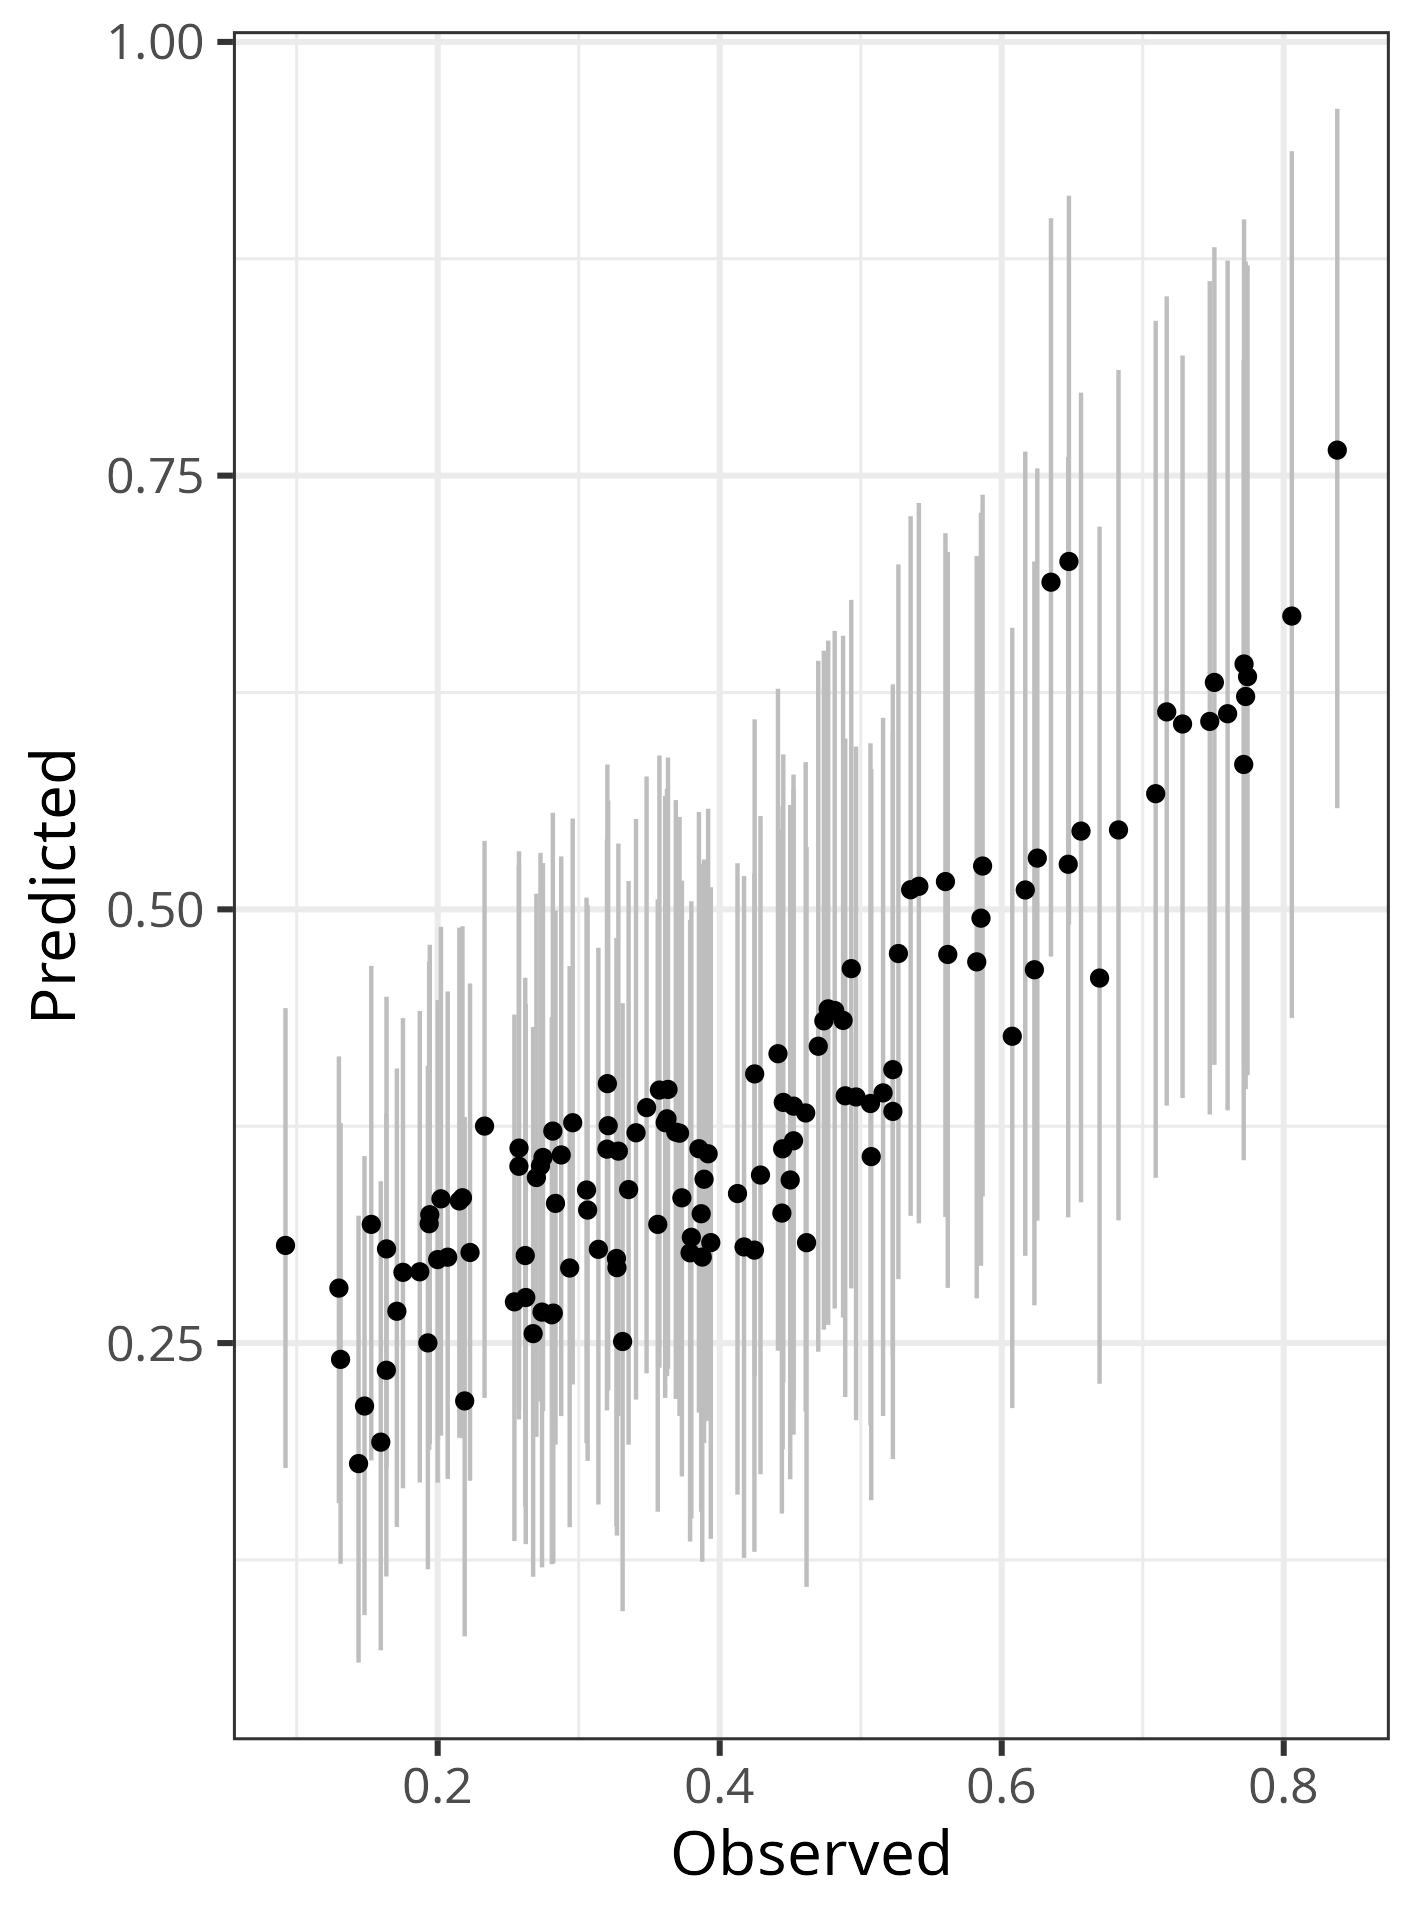
\includegraphics[width=29.11in]{README_files/figure-gfm/mobilityfitted} \caption{Fit of model to data.}\label{fig:mobilityfitted}
\end{figure}

\begin{figure}
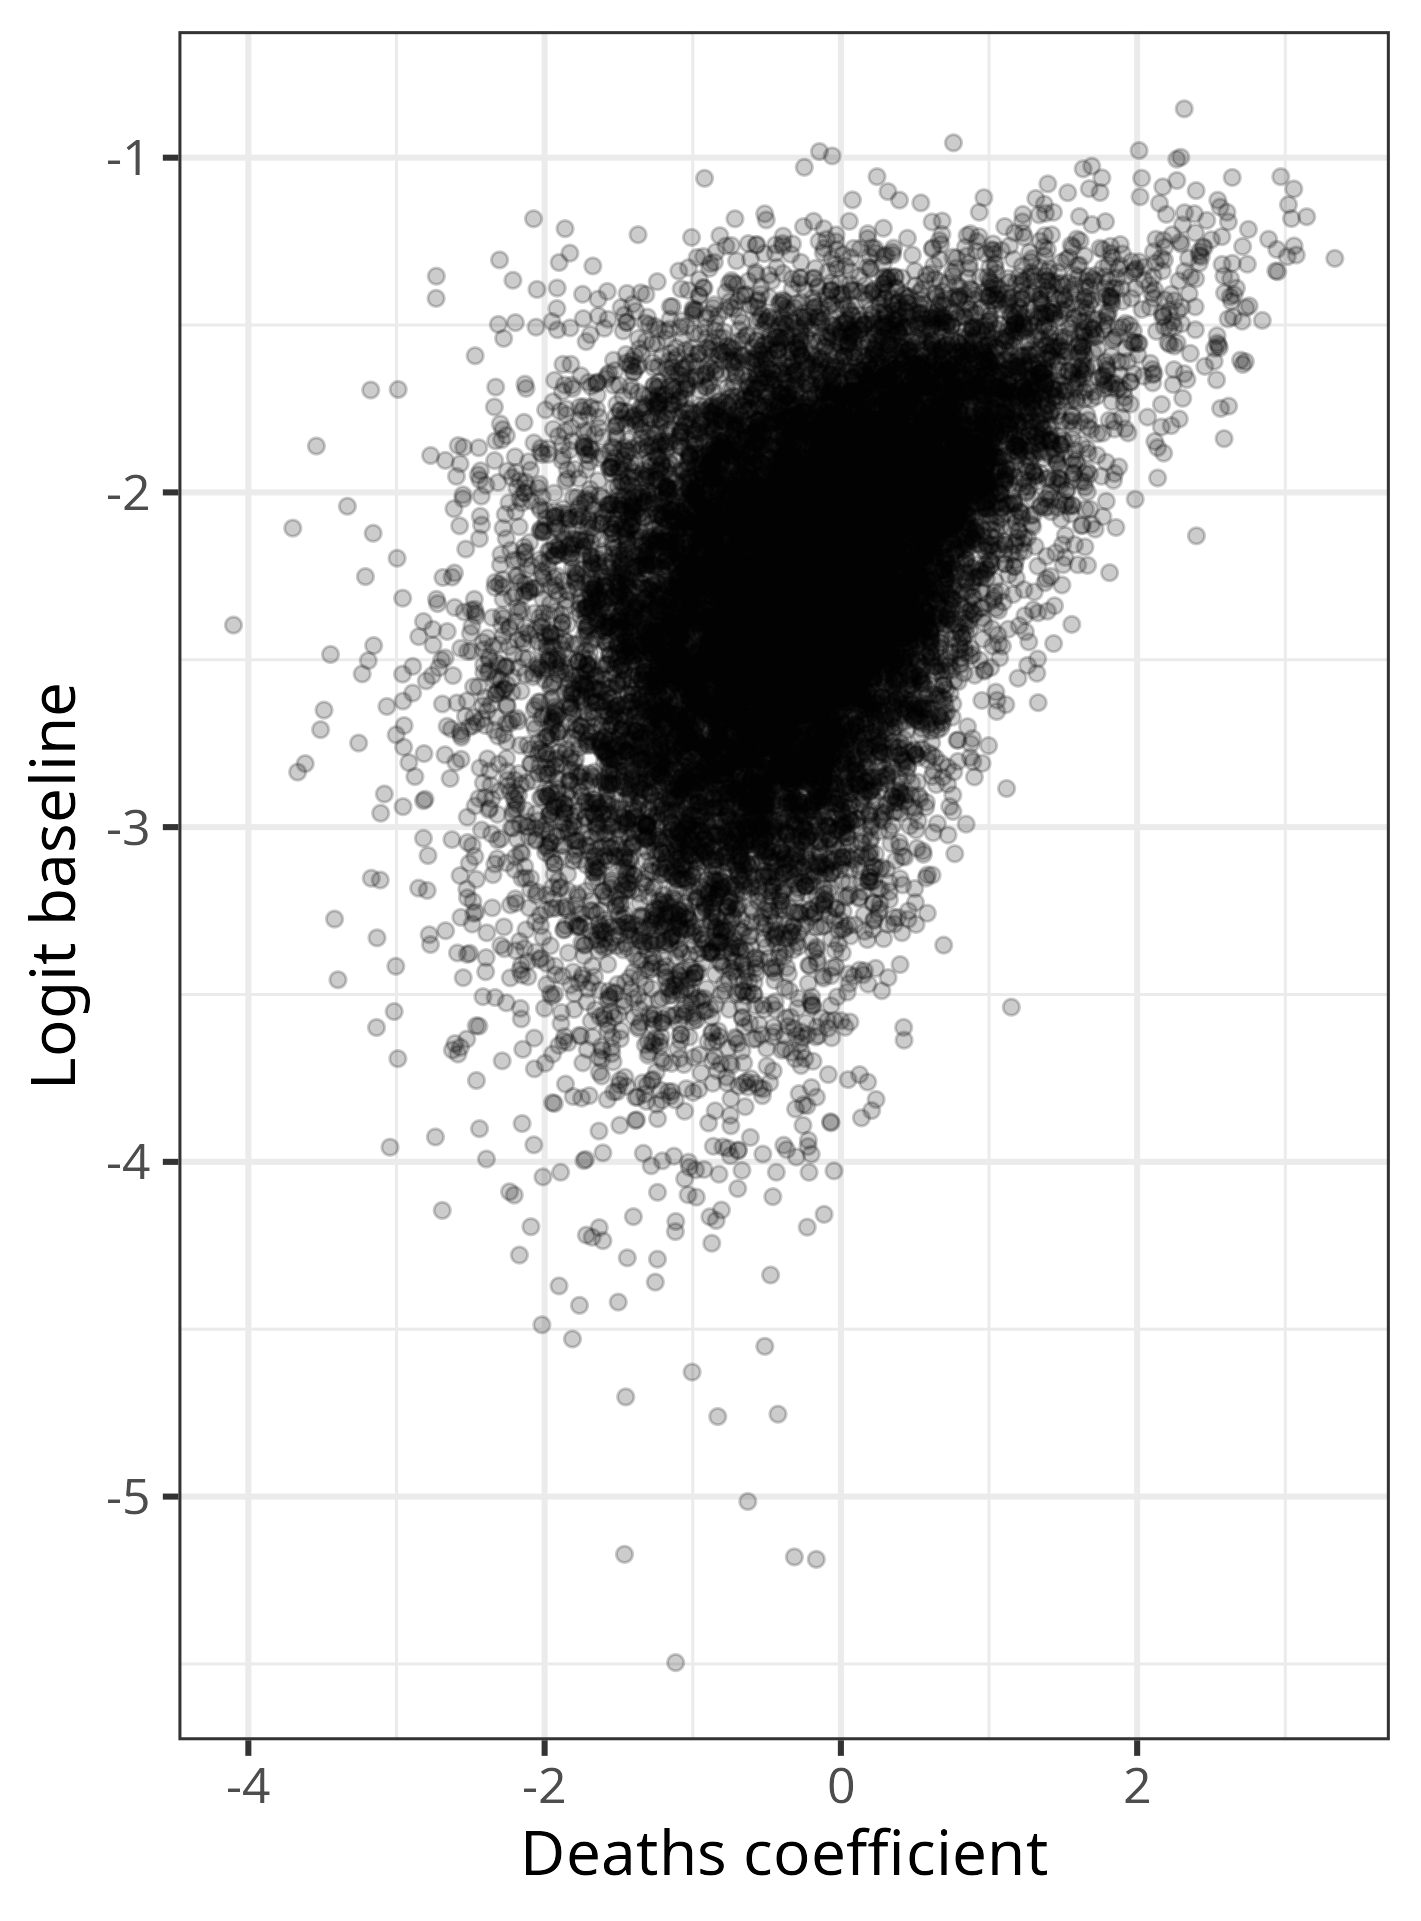
\includegraphics[width=29.11in]{README_files/figure-gfm/mobilityposterior} \caption{Posterior distribution for parameters $p^9$ and $p^8$.}\label{fig:mobilityposterior}
\end{figure}

\begin{figure}
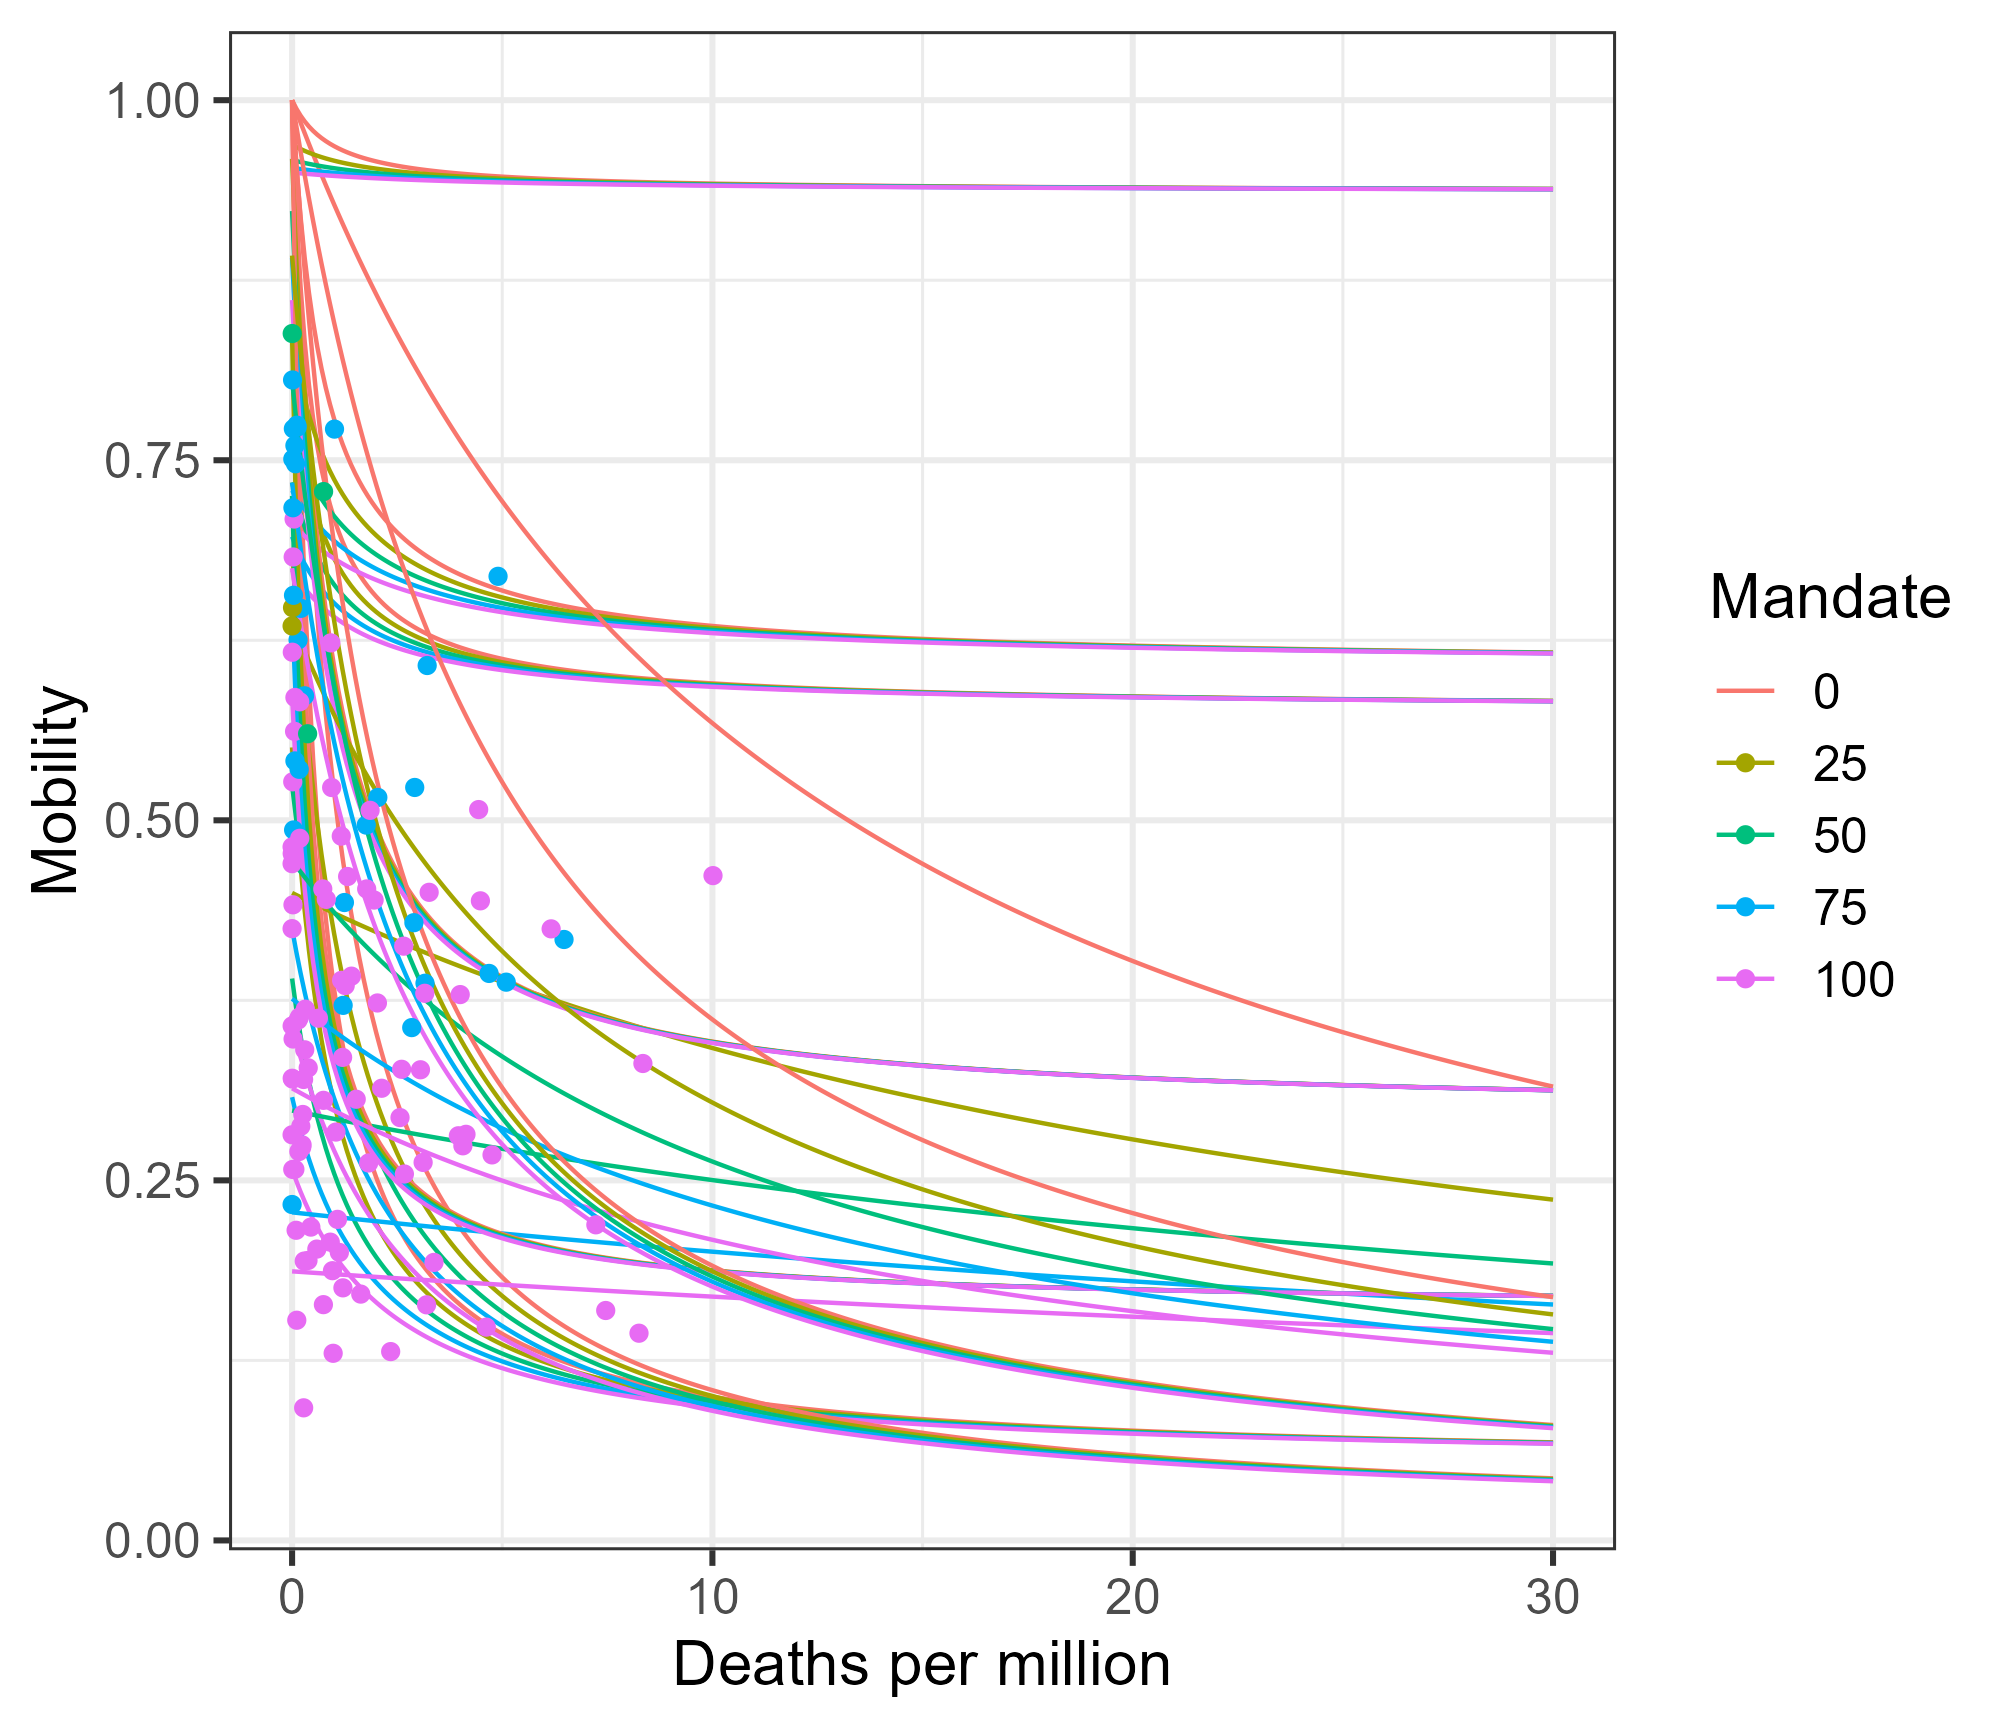
\includegraphics[width=29.11in]{README_files/figure-gfm/mobilitycurves} \caption{Sampled curves for four levels of mitigation. Data shown as points.}\label{fig:mobilitycurves}
\end{figure}

\hypertarget{self-isolating}{%
\subsection{Self isolating}\label{self-isolating}}

We assume that infectious people who know their status have a compliance \(p^1\sim\mathcal(U)(0,1)\) with the instruction to self isolate, starting one day into their infectious period. We assume constant infectiousness over time and that a fraction \(p^{26}\) of the symptomatic infectiousness is presymptomatic. Then the amount of infectiousness averted of symptomatic people is \(p^4=p^1(1-p^{26})\), who isolate due to the onset of symptoms. The fraction of asymptomatic cases identified by testing is \(p^2(t)\). We assume asymptomatic cases have the same probability to self isolate and that test results are returned after \(p^{17}\) days of infectiousness. Then the infectiousness that testing averts is \(p^3(t)=p^1p^2(t)\min(0,(T^{I^a:R}-p^{17})/T^{I^a:R})\).

\hypertarget{econ-model}{%
\section{Econ model}\label{econ-model}}

\hypertarget{configurations}{%
\subsection{Configurations}\label{configurations}}

\begin{longtable}[]{@{}
  >{\centering\arraybackslash}p{(\columnwidth - 12\tabcolsep) * \real{0.24}}
  >{\centering\arraybackslash}p{(\columnwidth - 12\tabcolsep) * \real{0.13}}
  >{\centering\arraybackslash}p{(\columnwidth - 12\tabcolsep) * \real{0.13}}
  >{\centering\arraybackslash}p{(\columnwidth - 12\tabcolsep) * \real{0.13}}
  >{\centering\arraybackslash}p{(\columnwidth - 12\tabcolsep) * \real{0.13}}
  >{\centering\arraybackslash}p{(\columnwidth - 12\tabcolsep) * \real{0.13}}
  >{\centering\arraybackslash}p{(\columnwidth - 12\tabcolsep) * \real{0.13}}@{}}
\caption{Economic configurations used to implement strategies. Values are the openness of the sector expressed as a percentage. Elimination values are taken from Australia. Lockdown and Economic Closures values are taken from the UK. School Closures values are taken from Indonesia. \label{tab:eccon}}\tabularnewline
\toprule
Sector & Heavy closures & Light closures & Heavy closures & Light closures & Heavy closures & Light closures \\
\midrule
\endfirsthead
\toprule
Sector & Heavy closures & Light closures & Heavy closures & Light closures & Heavy closures & Light closures \\
\midrule
\endhead
Agriculture, hunting, forestry & 86 & 100 & 86 & 88 & 100 & 100 \\
Fishing and aquaculture & 86 & 100 & 86 & 88 & 100 & 100 \\
Mining and quarrying, energy
producing products & 90 & 100 & 90 & 91 & 67 & 79 \\
Mining and quarrying,
non-energy producing products & 90 & 100 & 90 & 91 & 100 & 100 \\
Mining support service
activities & 90 & 100 & 90 & 91 & 100 & 100 \\
Food products, beverages and
tobacco & 70 & 100 & 70 & 94 & 100 & 100 \\
Textiles, textile products,
leather and footwear & 70 & 98 & 70 & 94 & 89 & 92 \\
Wood and products of wood and
cork & 70 & 98 & 70 & 94 & 100 & 95 \\
Paper products and printing & 70 & 98 & 70 & 94 & 100 & 98 \\
Coke and refined petroleum
products & 70 & 88 & 70 & 94 & 87 & 88 \\
Chemical and chemical products & 70 & 88 & 70 & 94 & 100 & 100 \\
Pharmaceuticals, medicinal
chemical and botanical
products & 70 & 88 & 70 & 94 & 100 & 100 \\
Rubber and plastics products & 70 & 88 & 70 & 94 & 87 & 100 \\
Other non-metallic mineral
products & 70 & 88 & 70 & 94 & 92 & 89 \\
Basic metals & 70 & 100 & 70 & 94 & 100 & 100 \\
Fabricated metal products & 70 & 100 & 70 & 94 & 90 & 100 \\
Computer, electronic and
optical equipment & 70 & 100 & 70 & 94 & 90 & 100 \\
Electrical equipment & 70 & 100 & 70 & 94 & 90 & 100 \\
Machinery and equipment, nec & 70 & 100 & 70 & 94 & 89 & 95 \\
Motor vehicles, trailers and
semi-trailers & 70 & 100 & 70 & 94 & 66 & 82 \\
Other transport equipment & 70 & 100 & 70 & 94 & 66 & 82 \\
Manufacturing nec; repair and
installation of machinery and
equipment & 70 & 98 & 70 & 94 & 98 & 100 \\
Electricity, gas, steam and
air conditioning supply & 89 & 97 & 89 & 100 & 94 & 94 \\
Water supply; sewerage, waste
management and remediation
activities & 92 & 97 & 92 & 98 & 100 & 100 \\
Construction & 56 & 94 & 56 & 92 & 95 & 95 \\
Wholesale and retail trade;
repair of motor vehicles & 64 & 100 & 64 & 100 & 92 & 97 \\
Land transport and transport
via pipelines & 63 & 100 & 63 & 82 & 83 & 100 \\
Water transport & 63 & 100 & 63 & 82 & 81 & 98 \\
Air transport & 63 & 18 & 63 & 82 & 16 & 42 \\
Warehousing and support
activities for transportation & 63 & 91 & 63 & 82 & 64 & 91 \\
Postal and courier activities & 63 & 91 & 63 & 82 & 64 & 91 \\
Accommodation and food service
activities & 10 & 92 & 10 & 85 & 77 & 91 \\
Publishing, audiovisual and
broadcasting activities & 88 & 100 & 88 & 91 & 100 & 100 \\
Telecommunications & 88 & 100 & 88 & 91 & 100 & 100 \\
IT and other information
services & 88 & 100 & 88 & 91 & 100 & 100 \\
Financial and insurance
activities & 94 & 100 & 94 & 96 & 100 & 100 \\
Real estate activities & 98 & 100 & 98 & 98 & 100 & 100 \\
Professional, scientific and
technical activities & 85 & 100 & 85 & 92 & 90 & 95 \\
Administrative and support
services & 66 & 90 & 66 & 80 & 90 & 95 \\
Public administration and
defence; compulsory social
security & 100 & 100 & 100 & 100 & 96 & 100 \\
Education & 10 & 100 & 10 & 100 & 10 & 10 \\
Human health and social work
activities & 75 & 100 & 75 & 92 & 100 & 100 \\
Arts, entertainment and
recreation & 55 & 94 & 55 & 71 & 90 & 96 \\
Other service activities & 54 & 94 & 54 & 83 & 90 & 96 \\
Activities of households as
employers; undifferentiated
goods- and services-producing
activities of households for
own use & 49 & 94 & 49 & 53 & 90 & 96 \\
\bottomrule
\end{longtable}

\hypertarget{impact-of-tourism}{%
\subsection{Impact of tourism}\label{impact-of-tourism}}

\hypertarget{food-and-accommodation-services-sector}{%
\subsubsection{Food and accommodation services sector}\label{food-and-accommodation-services-sector}}

As there is no ``tourism'' sector in the 45-sector classification we are using, to model the impact of changes to tourism, we identify the ``Food and accommodation services'' sector with tourism. This is imperfect. The correlation of their \% contributions to GDP is 0.64 and the order of magnitude is similar (1 to 7\% vs 2 to 10\% of GDP). The other two sectors considered (Air transport and Arts, entertainment and recreation) have little correlation with tourism in terms of \% of GDP. (See Figure \ref{fig:pairs}.)

\begin{figure}

{\centering 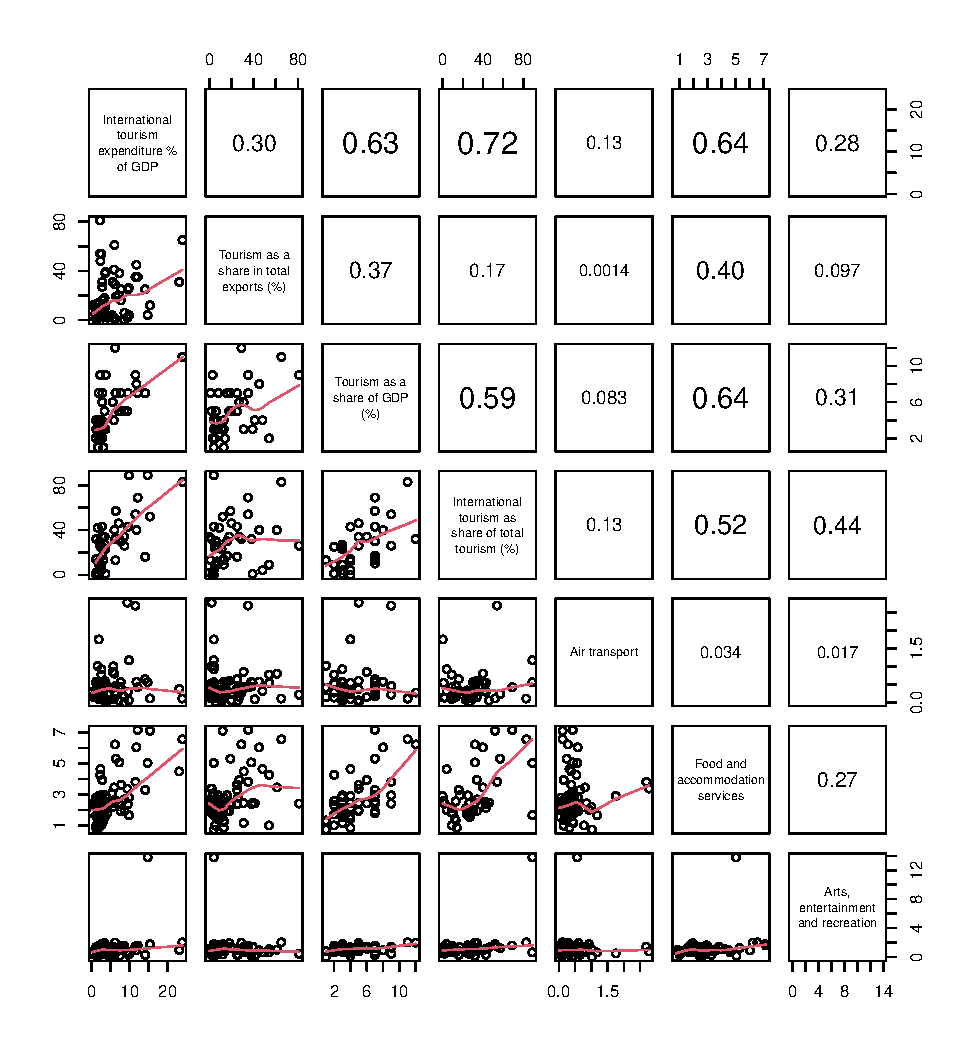
\includegraphics{README_files/figure-latex/pairs-1} 

}

\caption{Correlations between tourism-related data. First: https://www.unwto.org/tourism-statistics/key-tourism-statistics. Second to fourth: https://www.unwto.org/tourism-data/international-tourism-and-covid-19. Fifth to seventh: OECD.}\label{fig:pairs}
\end{figure}

\newpage

\hypertarget{sector-shrinkage-as-a-result-of-the-pandemic}{%
\subsubsection{Sector shrinkage as a result of the pandemic}\label{sector-shrinkage-as-a-result-of-the-pandemic}}

For many countries, tourism was reduced in the COVID-19 pandemic not because of domestic mandates but because of reduced international travel. Therefore, the fraction of tourism that comes from abroad is a factor that can determine the impact of a pandemic on a country's GDP potentially independently of what happens within the country. (A useful model extension would be to include some dependence on country factors, e.g.~case numbers.)

We model mitigation via business closures, which are mandated by sector. We represent openness with values \(x\) which range from 0 to 1, 1 representing maximum openness. To capture the impact of reduced international travel, we set the maximum openness of the food and accommodation services sector to be limited by international tourism as:

\begin{verbatim}
x = \min\{\hat{x}, 1+ b(c-1)\}
\end{verbatim}

where \(`\hat{x}`\) is the openness of the sector according to the schedule (i.e.~the mitigation strategy), \(b\) is the proportion of tourism that is international, and \(c\) is the fraction international tourism reduces to as a consequence of the pandemic. I.e. the tourism remaining is the domestic (\(1-b\)) plus that that comes in from abroad (\(bc\)).

Therefore, the contribution of the GVA of the food and accommodation services sector is limited either by the pandemic, or by the mitigation measures - whichever is lower.

\hypertarget{loss-of-international-tourists}{%
\subsubsection{Loss of international tourists}\label{loss-of-international-tourists}}

We model the distribution of \(c\) using data from 2020 (Figure \ref{fig:tourismhist}, bottom-right plot). We fit to it a log-normal distribution, and find mean value -1.39 and standard deviation 0.39 (Figure \ref{fig:ytd}). We use these values as inputs for all country models.

\begin{figure}

{\centering 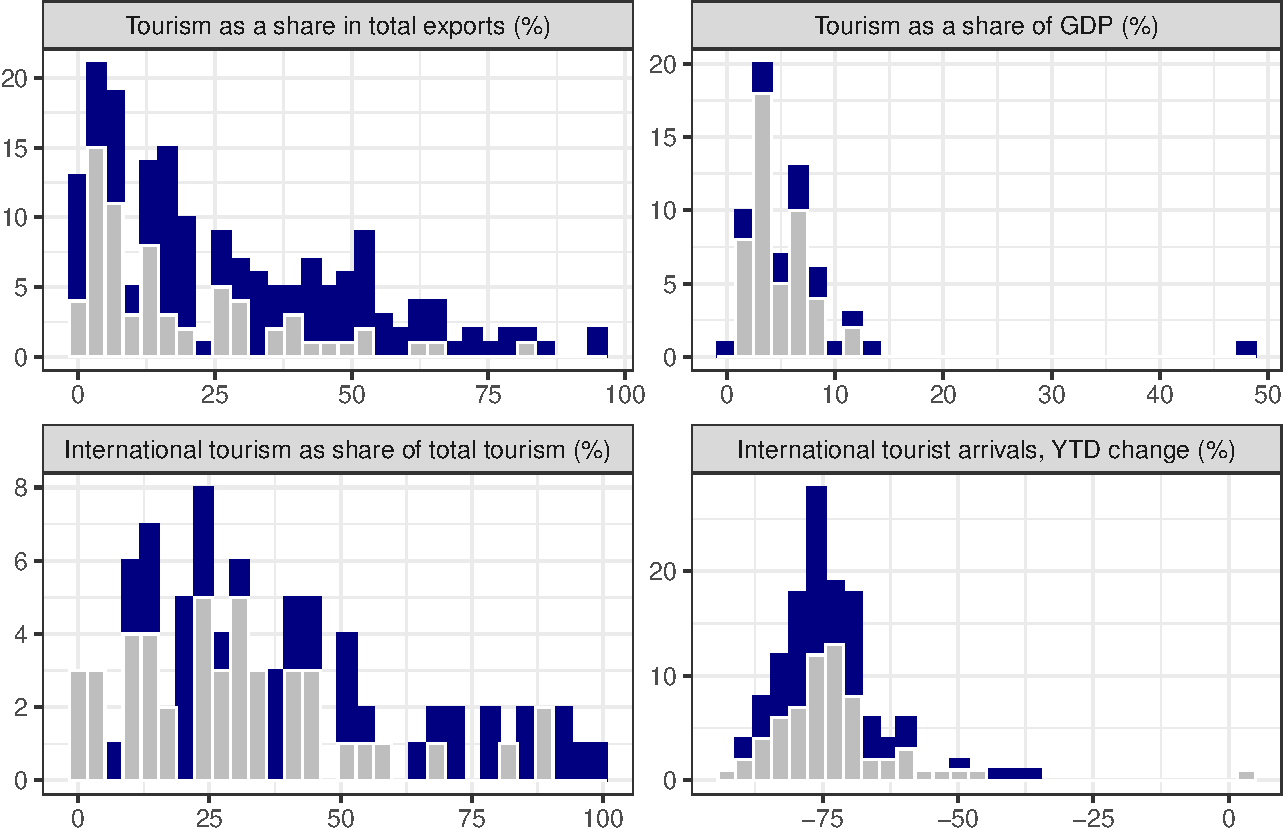
\includegraphics{README_files/figure-latex/tourismhist-1} 

}

\caption{Distributions of tourism-related data from https://www.unwto.org/tourism-data/international-tourism-and-covid-19. In grey are the subset of countries for which we have GVA data by sector.}\label{fig:tourismhist}
\end{figure}

\begin{figure}

{\centering 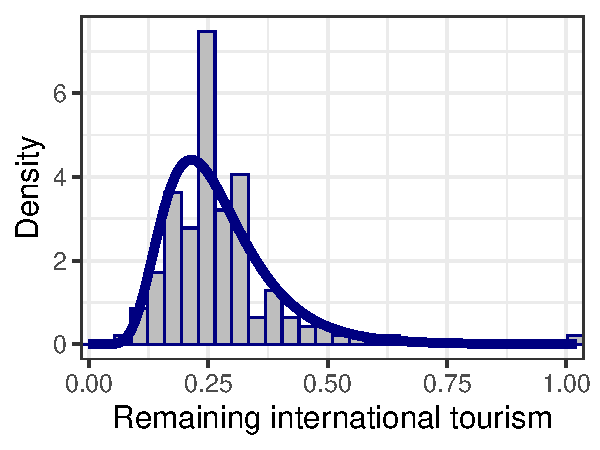
\includegraphics{README_files/figure-latex/ytd-1} 

}

\caption{Fit of log-normal distribution to loss-of-tourism data.}\label{fig:ytd}
\end{figure}

\newpage

\hypertarget{dependence-on-international-tourism}{%
\subsubsection{Dependence on international tourism}\label{dependence-on-international-tourism}}

We model \(b\) as a function of the share of GDP that comes from the sector. Note that the data we have for this are biased towards high-income countries.

We write

\[b\sim\text{Beta}(\alpha(z),\beta(z))\]

where \(z\) is the fraction of GDP coming from the Food and accommodation sector. We learn three parameters \(p^5\), \(p^6\) and \(p^7\) to best fit the relationship between \(z\) and \(b\) in countries we have observations for:

\[p^5 = \alpha(z)+\beta(z)\]

\[p^6 z + p^7 = \frac{\alpha(z)}{\alpha(z)+\beta(z)}\]

Here, \(p^5\) controls the variance of the distribution and \(p^6\) and \(p^7\) the linear relationship between \(z\) and \(b\). Using an optimisation routine in R we find \(p^5=5.93\), \(p^6=3.66\) and \(p^7=0.099\). Results are shown in Figure \ref{fig:sectortourism}. We use these values as inputs for all country models.

\begin{fignos:no-prefix-figure-caption}

\begin{figure}
\centering
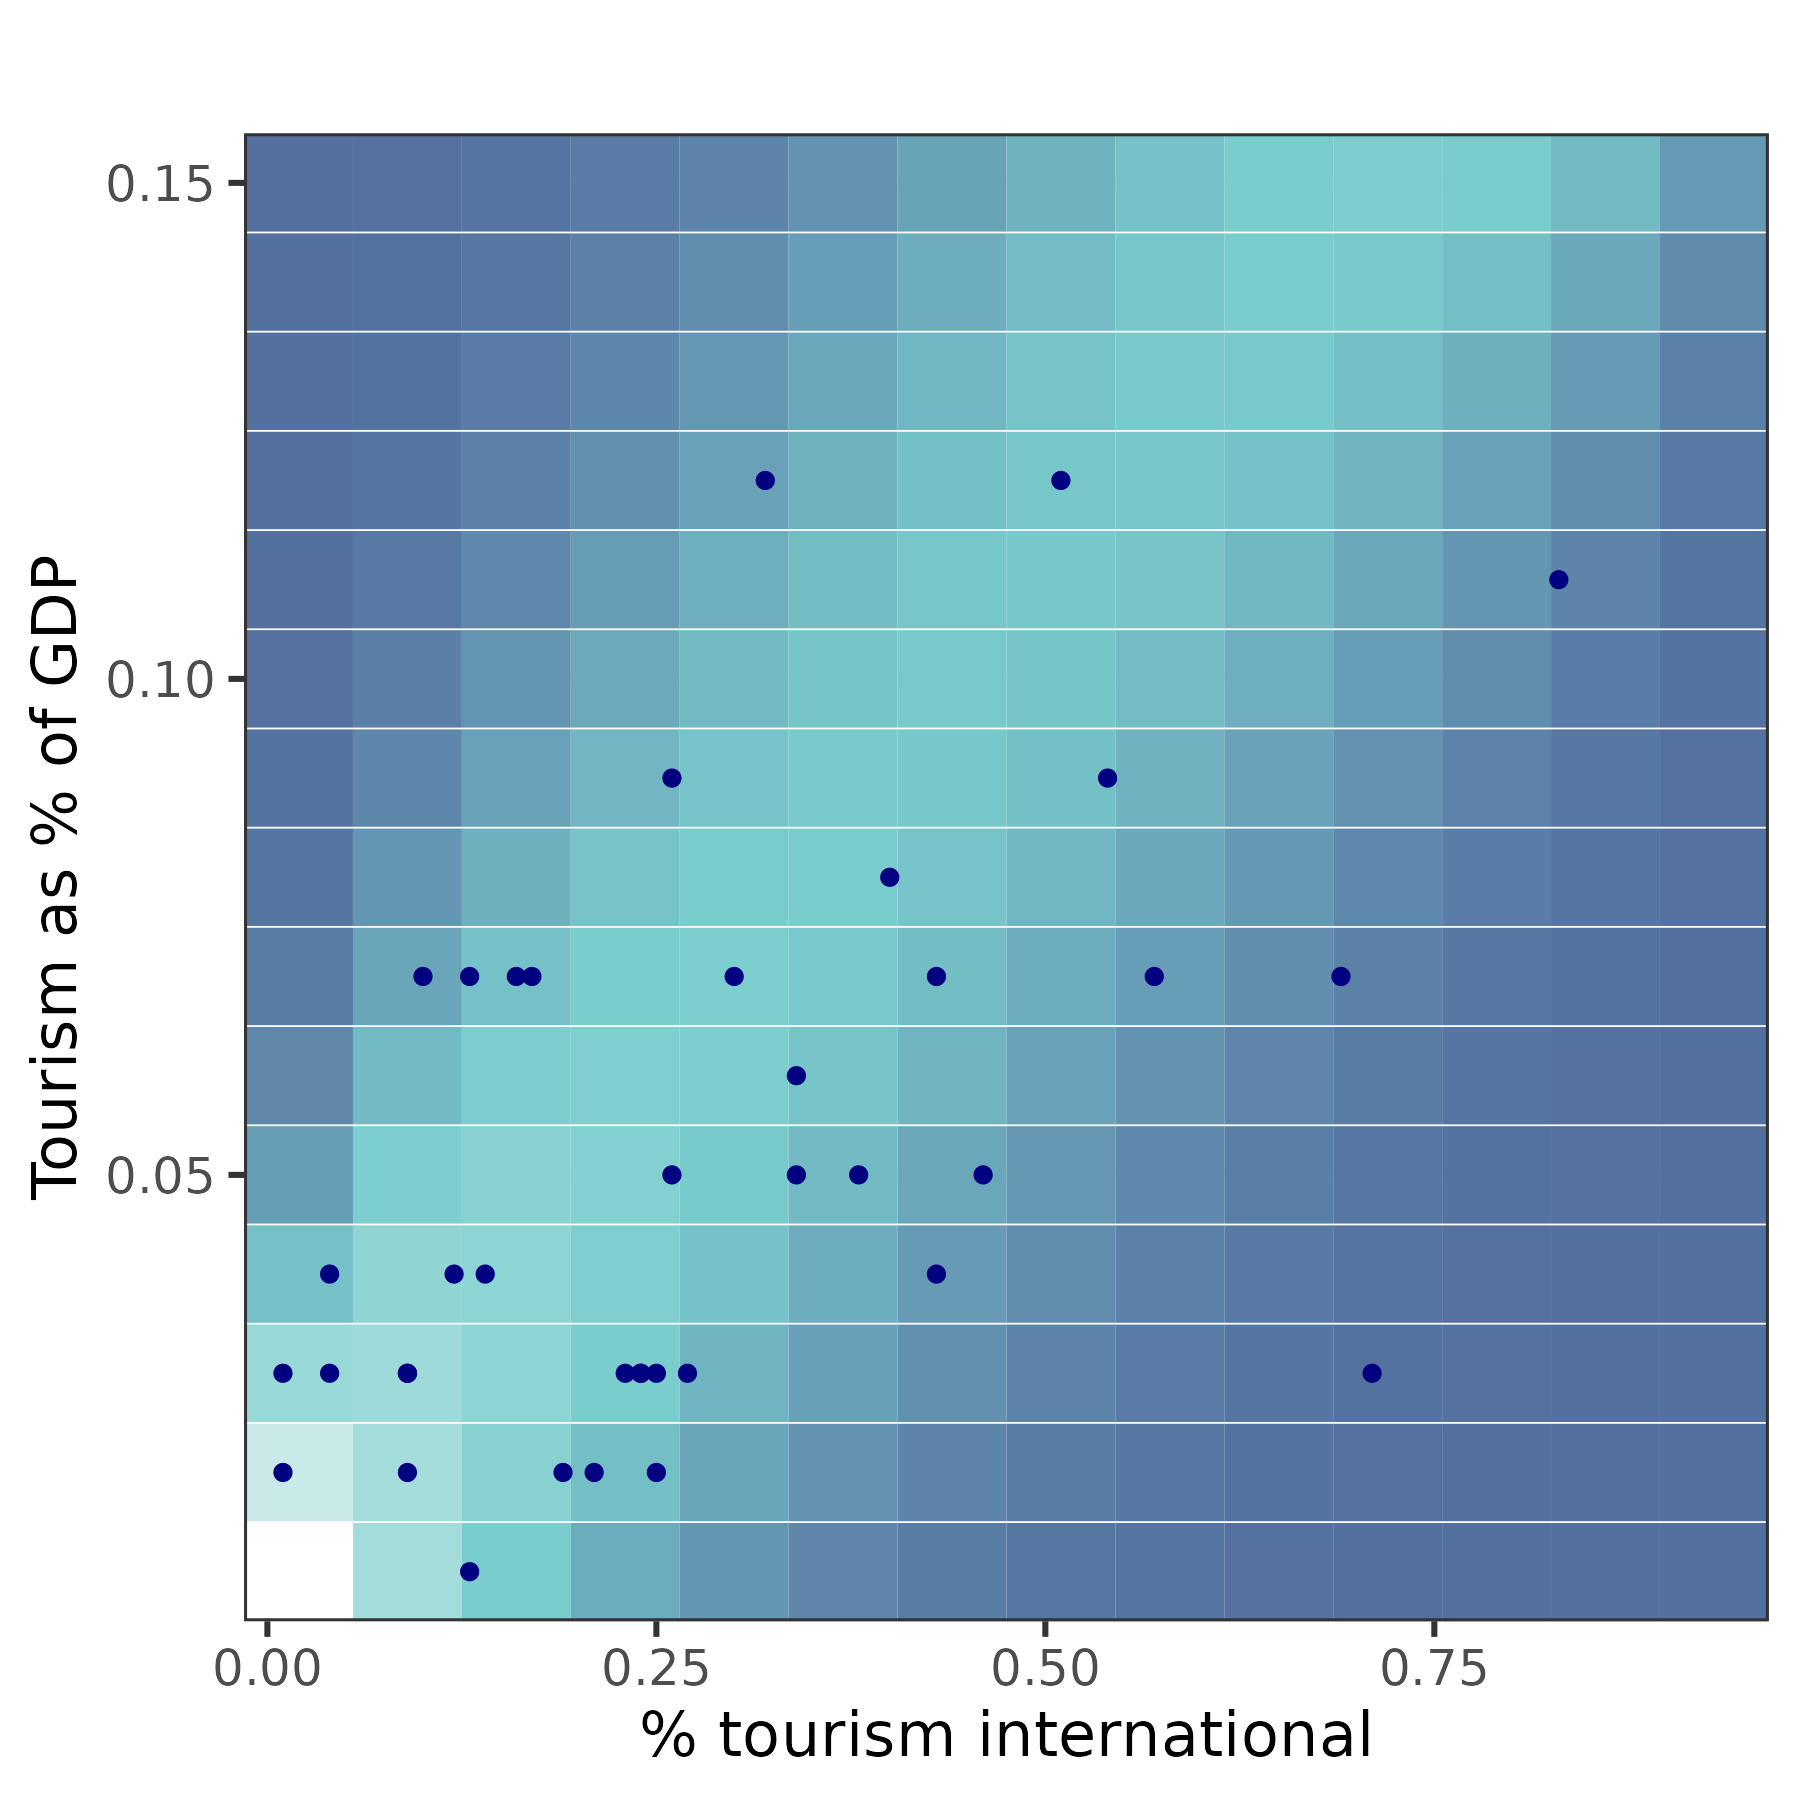
\includegraphics[width=0.6\textwidth,height=\textheight]{figures/sectortourism.png}
\caption{\label{fig:sectortourism} Predicting the percentage of tourism that comes from abroad as a function of the size of the sector. Each row represents a beta distribution whose mean is determined by the size of the sector (z). Blue points show the data we have available (grey bars in Figure \ref{fig:tourismhist}).}
\end{figure}

\end{fignos:no-prefix-figure-caption}

\newpage

\hypertarget{remote-working}{%
\subsection{Remote working}\label{remote-working}}

For each sector in each country, we have the 90\% interval for the proportion of people who can work from home from (Gottlieb et al. 2021). We assume that the value we sample within the range is related to internet infrastructure, so that a low value in one sector implies low values in all sectors. We:

\begin{itemize}
\tightlist
\item
  take the subset of countries in the income group (LLMIC / UMIC / HIC);
\item
  take the minimum of the lower bounds by sector (5\%);
\item
  take the maximum of the upper bounds by sector (95\%);
\item
  sample from a uniform distribution between these bounds, taking the same quantile for each sector.
\end{itemize}

\hypertarget{parametric-distributions}{%
\section{Parametric distributions}\label{parametric-distributions}}

\begin{longtable}[]{@{}
  >{\centering\arraybackslash}p{(\columnwidth - 8\tabcolsep) * \real{0.33}}
  >{\centering\arraybackslash}p{(\columnwidth - 8\tabcolsep) * \real{0.17}}
  >{\centering\arraybackslash}p{(\columnwidth - 8\tabcolsep) * \real{0.17}}
  >{\centering\arraybackslash}p{(\columnwidth - 8\tabcolsep) * \real{0.16}}
  >{\centering\arraybackslash}p{(\columnwidth - 8\tabcolsep) * \real{0.16}}@{}}
\caption{Parameter distributions. \label{tab:paramdist}}\tabularnewline
\toprule
Parameter & Income group & Distribution & Parameter 1 & Parameter 2 \\
\midrule
\endfirsthead
\toprule
Parameter & Income group & Distribution & Parameter 1 & Parameter 2 \\
\midrule
\endhead
internet coverage & LLMIC & Beta & 1.78 & 3.11 \\
internet coverage & UMIC & Beta & 14.32 & 6.44 \\
internet coverage & HIC & Beta & 9.57 & 1.39 \\
remaining international
tourism & all & Log normal & -1.39 & 0.39 \\
Labour share of GVA & LLMIC & Beta & 5.09 & 4.51 \\
Labour share of GVA & UMIC & Beta & 7.06 & 8.18 \\
Labour share of GVA & HIC & Beta & 7.97 & 6.87 \\
Hospital capacity & LLMIC & Gamma & 1.3 & 20.2 \\
Hospital capacity & UMIC & Gamma & 1.73 & 40.73 \\
Hospital capacity & HIC & Gamma & 2.05 & 46.57 \\
Public transport fraction & LLMIC & Beta & 4.88 & 3.65 \\
Public transport fraction & UMIC & Beta & 2.06 & 2.59 \\
Public transport fraction & HIC & Beta & 3.23 & 11.65 \\
tourism P1+P2 & all & NA & 6.73 & NA \\
Tourism to international & all & NA & 4.14 & 0.05 \\
pupil teacher ratio & LLMIC & Gamma & 9.15 & 0.32 \\
pupil teacher ratio & UMIC & Gamma & 13.29 & 0.82 \\
pupil teacher ratio & HIC & Gamma & 14.53 & 1.17 \\
school1 fraction & all & Beta & 2.14 & 3.38 \\
school2 fraction & all & Beta & 13.23 & 10.85 \\
work fraction & all & Beta & 11.11 & 13.82 \\
hospitality1 fraction & all & Beta & 21.08 & 381.2 \\
hospitality2 fraction & all & Beta & 3.71 & 88.67 \\
hospitality3 fraction & all & Beta & 19.44 & 149.4 \\
hospitality4 fraction & all & Beta & 7.69 & 62.33 \\
hospitality age1 & all & NA & 0.63 & 0.09 \\
hospitality age2 & all & NA & 0.57 & 0.06 \\
hospitality age3 & all & NA & 0.85 & 0.08 \\
hospitality age4 & all & NA & 0.56 & 0.41 \\
\bottomrule
\end{longtable}

\hypertarget{hospital-capacity}{%
\subsection{Hospital capacity}\label{hospital-capacity}}

\begin{fignos:no-prefix-figure-caption}

\begin{figure}
\centering
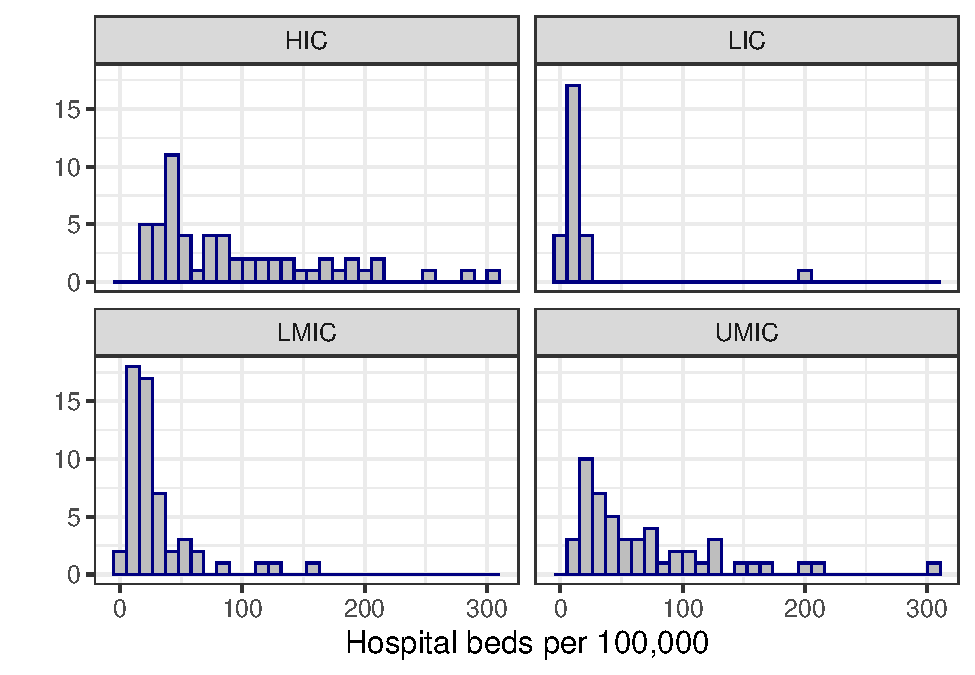
\includegraphics{README_files/figure-latex/hmax-1.pdf}
\caption{\label{fig:hmax}Hospital capacity: available beds minus usual occupancy.}
\end{figure}

\end{fignos:no-prefix-figure-caption}

We model these values with gamma distributions. For LLMICs, we have parameters 1.3 and 0.05. For UMICs, we have parameters 1.73 and 0.02. For HICs, we have parameters 2.05 and 0.02. (Data sources: World Bank (beds); OECD, WHO euro (bed occupancy rates).)

\hypertarget{labour-share-of-gva}{%
\subsection{Labour share of GVA}\label{labour-share-of-gva}}

We estimate the average annual income per working-age adult as the total GVA multiplied by the fraction of GVA that goes to labour divided by the number of working-age adults. For the fraction of GVA that goes to labour we use PWT estimates from 2011 (Figure \ref{fig:labsh}).

\begin{fignos:no-prefix-figure-caption}

\begin{figure}
\centering
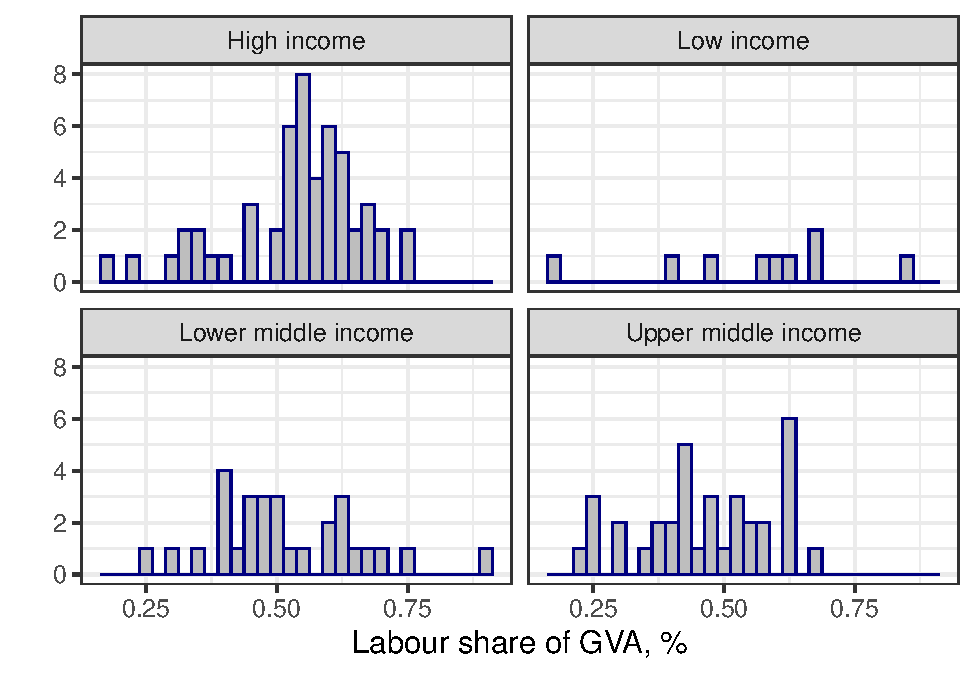
\includegraphics{README_files/figure-latex/labsh-1.pdf}
\caption{\label{fig:labsh}Fraction of GVA that goes to labour (PWT, 2011).}
\end{figure}

\end{fignos:no-prefix-figure-caption}

We model these values with Beta distributions. For LLMICs, we have parameters 5.09 and 4.51. For UMICs, we have parameters 7.06 and 8.18. For HICs, we have parameters 7.97 and 6.87.

\hypertarget{vaccine-administration}{%
\subsection{Vaccine administration}\label{vaccine-administration}}

\begin{fignos:no-prefix-figure-caption}

\begin{figure}
\centering
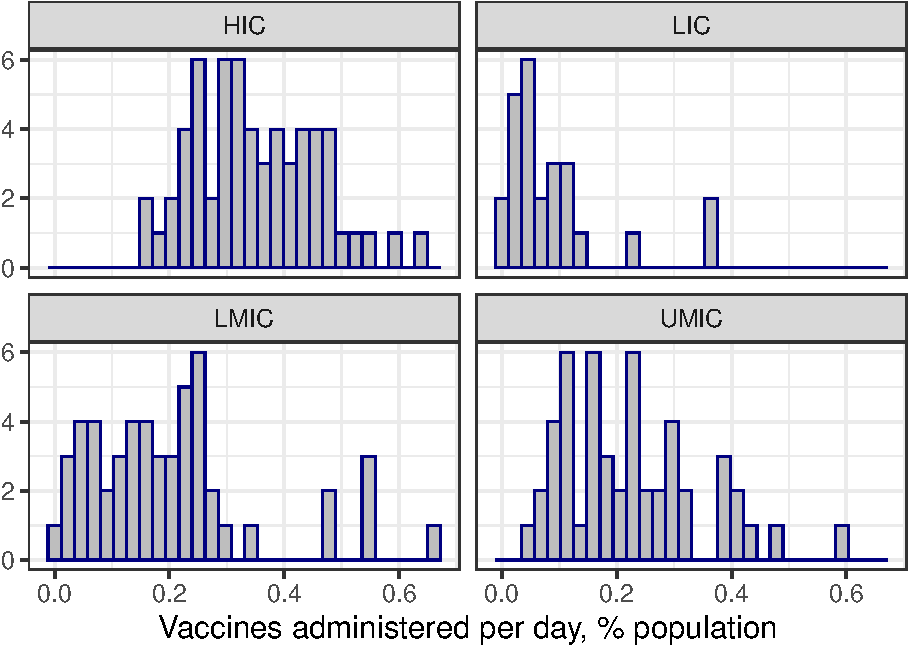
\includegraphics{README_files/figure-latex/vaxrate-1.pdf}
\caption{\label{fig:vaxrate}Vaccines administered per day, on average, in each country as a percent of population. Data source: fully vaccinated people from OWID (2022).}
\end{figure}

\end{fignos:no-prefix-figure-caption}

\newpage

\hypertarget{notation}{%
\section{Notation}\label{notation}}

In general in this notation, subscripts are indices, and superscripts are never indices but instead define new labels. In particular, note that numerical superscripts are attached to letters \(k\) for rates and \(p\) for parameters. Where a power is applied to one of these letters, the letter will be enclosed in parentheses for clarity.

\begin{longtable}[]{@{}
  >{\centering\arraybackslash}p{(\columnwidth - 6\tabcolsep) * \real{0.20}}
  >{\centering\arraybackslash}p{(\columnwidth - 6\tabcolsep) * \real{0.33}}
  >{\centering\arraybackslash}p{(\columnwidth - 6\tabcolsep) * \real{0.16}}
  >{\centering\arraybackslash}p{(\columnwidth - 6\tabcolsep) * \real{0.32}}@{}}
\caption{Capital letters}\tabularnewline
\toprule
Letter & Script & Subscript & Superscript \\
\midrule
\endfirsthead
\toprule
Letter & Script & Subscript & Superscript \\
\midrule
\endhead
\(A\) & & & \\
\(B\) & & & \\
\(C\) & consumption & & community (contacts) \\
\(D\) & COMPARTMENT: Died & & related to death state \\
\(E\) & COMPARTMENT: Exposed & & related to exposed state \\
\(F\) & & & \\
\(G\) & & & \\
\(GDP\) & GDP & & \\
\(H\) & COMPARTMENT: Hospitalised & & related to hospitalised state \\
\(H_{\text{max}}\) & hospital capacity & & \\
\(I\) & Infectious & & \\
\(I^{a}\) & COMPARTMENT: Infectious
asymptomatic & & related to asymptomatic state \\
\(I^{s}\) & COMPARTMENT: Infectious
symptomatic & & related to symptomatic state \\
\(J\) & & MAX: strata & \\
\(K\) & Loss (cost calculation) & & \\
\(L\) & number of people by sector
(workforce in place) & & \\
\(M^{\text{com}}\) & CONTACTS: community & & \\
\(M^{\text{home}}\) & CONTACTS: community, home & & \\
\(M^{\text{CC}}\) & CONTACTS: community, customers & & \\
\(M^{\text{trav}}\) & CONTACTS: community, public
transport & & \\
\(M^{\text{sch}}\) & CONTACTS: community, school & & \\
\(M^{\text{WW}}\) & CONTACTS: work, workers & & \\
\(M^{\text{WC}}\) & CONTACTS: work, worker to
customer & & \\
\(M^{\text{CW}}\) & CONTACTS: work, customer to
worker & & \\
\(M\) & CONTACTS: total & & \\
\(\tilde{M}\) & Total contacts by five-year
age bands & & \\
\(\hat{M}\) & Total contacts by DAEDALUS age
groups & & \\
\(N\) & number of people by stratum & & \\
\(\tilde{N}\) & Number of people by five-year
age bands & & \\
\(\hat{N}\) & Number of people in DAEDALUS
age groups & & \\
\(O\) & -- & & \\
\(P\) & (probability) & & \\
\(Q\) & & & \\
\(R\) & COMPARTMENT: Recovered & & related to recovered state \\
\(R_0\) & Basic reproduction number & & \\
\(R_t\) & Effective reproduction number & & \\
\(S\) & COMPARTMENT: Susceptible & MAX: sectors & \\
\(S^{c}\) & COMPARTMENT: Susceptible
seroconverting & & \\
\(T^c\) & duration from vaccination to
protection & & \\
\(T^H\) & duration in hospital & & \\
\(T^{H:D}\) & duration in hospital given
death & & \\
\(T^{H:R}\) & duration in hospital given
recovery & & \\
\(T^{I^a}\) & duration asymptomatic & & \\
\(T^{I^s}\) & duration symptomatic & & \\
\(T^{I^s:H}\) & duration symptomatic given
hospitalised & & \\
\(T^{I^s:R}\) & duration symptomatic given
recovery & & \\
\(T^{E:I}\) & latent period & & \\
\(U\) & & & \\
\(V\) & & MAX: vaccines & \\
\(W\) & & & worker (contacts) \\
\(X\) & & & \\
\(Y\) & GDP & MAX: years & \\
\(Y_0\) & max GDP & & \\
\(Z\) & & & \\
\bottomrule
\end{longtable}

\begin{longtable}[]{@{}
  >{\centering\arraybackslash}p{(\columnwidth - 6\tabcolsep) * \real{0.18}}
  >{\centering\arraybackslash}p{(\columnwidth - 6\tabcolsep) * \real{0.33}}
  >{\centering\arraybackslash}p{(\columnwidth - 6\tabcolsep) * \real{0.33}}
  >{\centering\arraybackslash}p{(\columnwidth - 6\tabcolsep) * \real{0.17}}@{}}
\caption{Lower-case letters}\tabularnewline
\toprule
Letter & Script & Subscript & Superscript \\
\midrule
\endfirsthead
\toprule
Letter & Script & Subscript & Superscript \\
\midrule
\endhead
\(a\) & & INDEX: age index, five-year
age bands & asymptomatic \\
\(b\) & proportion of tourism that is
international & & \\
\(c\) & fraction international tourism
reduces to as a consequence of
the pandemic & & seroconverting \\
\(d\) & deaths per million & & \\
\(e\) & government mandate & & \\
\(\text{ed}\) & & education sector (j index) & \\
\(f\) & functions: sd, hospitalisation & & \\
\(g\) & & INDEX: age index, DAEDALUS age
groups & \\
\(h\) & & INDEX: dummy index & \\
\(i\) & & & self isolating \\
\(j\) & & INDEX: stratum index & \\
\(k\) & state transition rates & & \\
\(l\) & life expectancy & & \\
\(m_J\) & number of strata & & \\
\(m_S\) & number of sectors & & \\
\(m_V\) & number of vaccines & & \\
\(m_Y\) & number of years in work & & \\
\(n\) & & & \\
\(o\) & -- & & \\
\(p\) & parameters & & \\
\(q\) & proportions working from home & & \\
\(r\) & discount rate & & \\
\(s\) & & & symptomatic \\
\(\text{school}\) & & student strata (j index) & \\
\(t\) & time (day) & & \\
\(u\) & dummy variable & INDEX: dummy index & \\
\(v\) & & INDEX: vaccination status & \\
\(w\) & & & \\
\(x\) & sector openness & & \\
\(y\) & GVA & INDEX: year & \\
\(z\) & fraction of GDP coming from
the Food and accommodation
sector & & \\
\bottomrule
\end{longtable}

\begin{longtable}[]{@{}
  >{\centering\arraybackslash}p{(\columnwidth - 2\tabcolsep) * \real{0.18}}
  >{\centering\arraybackslash}p{(\columnwidth - 2\tabcolsep) * \real{0.36}}@{}}
\caption{Greek letters}\tabularnewline
\toprule
Letter & Definition \\
\midrule
\endfirsthead
\toprule
Letter & Definition \\
\midrule
\endhead
\(\alpha\) & \\
\(\beta\) & transmission rate \\
\(\gamma\) & \\
\(\delta\) & \\
\(\epsilon\) & ratio transmission from
asymptomatic \\
\(\zeta\) & \\
\(\eta\) & vaccine effects \\
\(\theta\) & \\
\(\iota\) & \\
\(\kappa\) & \\
\(\lambda\) & \\
\(\mu\) & \\
\(\nu\) & growth rate \\
\(o\) & -- \\
\(\pi\) & \\
\(\rho\) & transmission modifier \\
\(\sigma\) & \\
\(\tau\) & max time \\
\(\upsilon\) & -- \\
\(\phi\) & \\
\(\chi\) & \\
\(\psi\) & \\
\(\omega\) & \\
\bottomrule
\end{longtable}

\begin{longtable}[]{@{}
  >{\centering\arraybackslash}p{(\columnwidth - 2\tabcolsep) * \real{0.15}}
  >{\centering\arraybackslash}p{(\columnwidth - 2\tabcolsep) * \real{0.46}}@{}}
\caption{Rates}\tabularnewline
\toprule
Letter & Definition \\
\midrule
\endfirsthead
\toprule
Letter & Definition \\
\midrule
\endhead
\(k^1\) & rate of infection \\
\(k^2\) & rate of onset of asymptomatic
infection \\
\(k^3\) & rate of recovery from
asymptomatic infection \\
\(k^4\) & rate of onset of symptomatic
infection \\
\(k^5\) & rate of recovery from
symptomatic infection \\
\(k^6\) & rate of hospitalisation \\
\(k^7\) & rate of recovery from
hospitalisation \\
\(k^8\) & rate of death from
hospitalisation \\
\(k^9\) & rate of vaccine seroconversion \\
\(k^{10}\) & vaccination rate \\
\(k^{11}\) & \\
\(k^{12}\) & rate of infection \\
\(k^{13}\) & \\
\(k^{14}\) & \\
\(k^{15}\) & \\
\(k^{16}\) & \\
\(k^{17}\) & \\
\(k^{18}\) & \\
\(k^{19}\) & rate of infection \\
\bottomrule
\end{longtable}

\begin{longtable}[]{@{}
  >{\centering\arraybackslash}p{(\columnwidth - 2\tabcolsep) * \real{0.22}}
  >{\centering\arraybackslash}p{(\columnwidth - 2\tabcolsep) * \real{0.46}}@{}}
\caption{Parameters}\tabularnewline
\toprule
Letter & Definition \\
\midrule
\endfirsthead
\toprule
Letter & Definition \\
\midrule
\endhead
\(p^{I^S}\) & probability to be symptomatic \\
\(\tilde{p}^H\) & Basic probability to be
hospitalised \\
\(p^H\) & Adjusted probability to be
hospitalised \\
\(\tilde{p}^D\) & Basic probability to die \\
\(p^D\) & Adjusted probability to die \\
\(p^1\) & Compliance with the
instruction to self isolate \\
\(p^2\) & fraction of cases identified
by testing \\
\(p^3\) & proportion of asymptomatic
infectiousness averted due to
self isolating \\
\(p^4\) & proportion of symptomatic
infectiousness averted due to
self isolating \\
\(p^5\) & tourism parameter \\
\(p^6\) & tourism parameter \\
\(p^7\) & tourism parameter \\
\(p^8\) & minimum mobility \\
\(p^9\) & deaths coefficient for
mobility \\
\(p^{10}\) & mandate coefficient for
mobility \\
\(p^{11}\) & mobility mixing parameter \\
\(p^{12}\) & present value of lost earnings \\
\(p^{13}\) & mean annual earnings \\
\(p^{14}\) & effective amount of education
lost per student \\
\(p^{15}\) & rate of return for one year of
education \\
\(p^{16}\) & relative effectiveness of
remote education \\
\(p^{17}\) & number of days from onset of
infectiousness to self
isolation \\
\(p^{18}\) & number of asymptomatic days
spent in self isolation per
day of infectiousness \\
\(p^{19}\) & number of symptomatic days
spent in self isolation per
day of infectiousness \\
\(p^{20}\) & number of days from onset of
symptoms to self isolation \\
\(p^{21}\) & public transport mode share \\
\(p^{22}\) & work absence, asymptomatic
(cost calculation) \\
\(p^{23}\) & work absence, symptomatic
(cost calculation) \\
\(p^{24}\) & school absence, asymptomatic
(cost calculation) \\
\(p^{25}\) & school absence, symptomatic
(cost calculation) \\
\(p^{26}\) & fraction of symptomatic
infectiousness that is
presymptomatic \\
\(p^{27}\) & hospitality openness \\
\bottomrule
\end{longtable}

\newpage

\hypertarget{refs}{}
\begin{CSLReferences}{1}{0}
\leavevmode\hypertarget{ref-Ananthapavan2021}{}%
Ananthapavan, Jaithri, Marj Moodie, Andrew J. Milat, and Rob Carter. 2021. {``{Systematic review to update `value of a statistical life' estimates for Australia}.''} \emph{International Journal of Environmental Research and Public Health} 18 (11). \url{https://doi.org/10.3390/ijerph18116168}.

\leavevmode\hypertarget{ref-Betthauser2023}{}%
Betthäuser, Bastian A, Anders M Bach-Mortensen, and Per Engzell. 2023. {``{A systematic review and meta-analysis of the evidence on learning during the COVID-19 pandemic}.''} \emph{Nature Human Behaviour} 7 (March). \url{https://doi.org/10.1038/s41562-022-01506-4}.

\leavevmode\hypertarget{ref-Beraud2015}{}%
Béraud, Guillaume, Sabine Kazmercziak, Philippe Beutels, Daniel Levy-Bruhl, Xavier Lenne, Nathalie Mielcarek, Yazdan Yazdanpanah, Pierre Yves Boëlle, Niel Hens, and Benoit Dervaux. 2015. {``{The French connection: The first large population-based contact survey in France relevant for the spread of infectious diseases}.''} \emph{PLoS ONE} 10 (7): 1--22. \url{https://doi.org/10.1371/journal.pone.0133203}.

\leavevmode\hypertarget{ref-Cutler2020}{}%
Cutler, David M., and Lawrence H. Summers. 2020. {``{The COVID-19 pandemic and the {\$}16 trillion virus}.''} \emph{JAMA} 324 (15). \url{https://doi.org/10.1257/pol.20170046}.

\leavevmode\hypertarget{ref-GlobalBurdenofDiseaseCollaborativeNetwork2021}{}%
Global Burden of Disease Collaborative Network. 2021. {``{Global Burden of Disease Study 2019 (GBD 2019) Reference Life Table}.''} Seattle, United States of America: Institute for Health Metrics; Evaluation (IHME).

\leavevmode\hypertarget{ref-Gottlieb2021}{}%
Gottlieb, Charles, Jan Grobovšek, Markus Poschke, and Fernando Saltiel. 2021. {``{Working from home in developing countries}.''} \emph{European Economic Review} 133: 103679. \url{https://doi.org/10.1016/j.euroecorev.2021.103679}.

\leavevmode\hypertarget{ref-Haw2020}{}%
Haw, David, Giovanni Forchini, Patrick Doohan, Paula Christen, Matteo Pianella, Rob Johnson, Sumali Bajaj, et al. 2022. {``{Optimizing social and economic activity while containing SARS-CoV-2 transmission using DAEDALUS}.''} \emph{Nature Computational Science} 2: 223--33. \url{https://doi.org/10.25561/83928}.

\leavevmode\hypertarget{ref-Jarvis2023}{}%
Jarvis, Christopher I, Pietro Coletti, Jantien A Backer, James D Munday, Christel Faes, Philippe Beutels, Christian L. Althaus, et al. 2023. {``{Social contact patterns following the COVID-19 pandemic: a snapshot of post-pandemic behaviour from the CoMix study}.''} \emph{MedRxiv}.

\leavevmode\hypertarget{ref-Moscoviz2022}{}%
Moscoviz, Laura, and David K Evans. 2022. {``{Learning loss and student dropouts during the COVID-19 pandemic: A review of the evidence two years after schools shut down}.''} Washington, DC: Center for Global Development.

\leavevmode\hypertarget{ref-Patrinos2023}{}%
Patrinos, Harry Anthony. 2023. {``{The longer students were out of school, the less they learned}.''} \emph{Journal of School Choice} 17 (2): 161--75. \url{https://doi.org/10.1080/15582159.2023.2210941}.

\leavevmode\hypertarget{ref-Prem2021}{}%
Prem, Kiesha, Kevin van Zandvoort, Petra Klepac, Rosalind M. Eggo, Nicholas G. Davies, Alex R. Cook, and Mark Jit. 2021. {``{Projecting contact matrices in 177 geographical regions: An update and comparison with empirical data for the COVID-19 era}.''} \emph{PLoS Computational Biology} 17 (7). \url{https://doi.org/10.1371/journal.pcbi.1009098}.

\leavevmode\hypertarget{ref-Psacharopoulos2021a}{}%
Psacharopoulos, George, Victoria; Collis, and Patrinos. 2021. {``{The COVID-19 Cost of School Closures in Earnings and Income across the World}.''} \emph{Comparative Education Review} 65 (2).

\leavevmode\hypertarget{ref-Robinson2021}{}%
Robinson, Lisa A., Ryan Sullivan, and Jason F. Shogren. 2021. {``{Do the benefits of COVID-19 policies exceed the costs? Exploring uncertainties in the age--VSL relationship}.''} \emph{Risk Analysis} 41 (5): 761--70. \url{https://doi.org/10.1111/risa.13561}.

\leavevmode\hypertarget{ref-Walker2020}{}%
Walker, Patrick G. T., Charles Whittaker, Oliver J. Watson, Marc Baguelin, Peter Winskill, Arran Hamlet, Bimandra A. Djafaara, et al. 2020. {``{The impact of COVID-19 and strategies for mitigation and suppression in low- and middle-income countries}.''} \emph{Science} 369 (6502): 413--22. \url{https://doi.org/10.1126/science.abc0035}.

\end{CSLReferences}

\end{document}
